
\documentclass[fleqn,usenatbib]{mnras}

\usepackage[T1]{fontenc}
\usepackage{newtxtext,newtxmath}
\usepackage{graphicx}
\graphicspath{{./}{../}}
\usepackage{amsmath}
\usepackage{bm}
\usepackage{booktabs}
\usepackage{siunitx}

% ---- convenient shorthands (math mode only where needed) ----
\newcommand{\nHH}{n_{\mathrm{H_2}}}
\newcommand{\logn}{\log_{10}(n_{\mathrm{H_2}})}
\newcommand{\Gzero}{G_0}
\newcommand{\fshield}{f_{\mathrm{H_2}}}
\newcommand{\enssp}{\textsc{ens\_sp}}
\newcommand{\dex}{\,\text{dex}}
\newcommand{\Rsq}{R^2}

% ============================================================
\title[ML surrogates for H\(_2\) density in ISM simulations]%
      {Machine learning surrogates for molecular hydrogen density in
       three-dimensional interstellar medium simulations:
       multi-scale spatial features outperform volumetric neural networks
       under out-of-distribution generalisation}

\author[D.~H.~Breger]{Daniel H.~Breger$^{1}$\thanks{E-mail: danielbreger@campus.technion.ac.il}
\\
$^{1}$Department of Physics, Technion,
Haifa, Israel}

\date{}
\pubyear{2026}

% ============================================================
\begin{document}

\label{firstpage}
\pagerange{\pageref{firstpage}--\pageref{lastpage}}
\maketitle

% ============================================================
\begin{abstract}
The molecular hydrogen number density $\nHH$ is a fundamental quantity
in interstellar-medium physics, yet computing it self-consistently in
three-dimensional simulations requires solving time-dependent
non-equilibrium chemistry coupled to radiative transfer, an expense that
severely limits the resolution and UV-parameter coverage of modern
calculations. We train a machine learning surrogate to predict
$\logn$ from 15 local physical properties at each cell of a $128^3$
simulation grid, and evaluate it under a stringent
leave-one-$\Gzero$-out cross-validation protocol in which each fold
withholds an entire simulation at a UV field strength $\Gzero$ (Habing
units) absent from training. Our data set comprises seven UV-only
chemistry simulations at $\Gzero \in \{0.1, 0.2, 0.4, 0.8, 1.6, 3.2,
6.4\}$ Habing, totalling 14,680,064 cells. The principal methodological
contribution is the replacement of a 3D U-Net convolutional neural
network with multi-scale spatial neighbourhood features: uniform
box-filter averages of all 15 physical fields computed at kernel sizes
$3^3$, $5^3$, and $7^3$ voxels via separable convolution in
$\approx$30\,s. Adding these 45 spatial features to a gradient-boosted
tree model improves the mean log-space $\Rsq$ from 0.886 to 0.924 in a
single deterministic preprocessing step. An equal-weight ensemble of
XGBoost and a wide fully-connected MLP, each trained on the resulting
60-dimensional feature set (\enssp), achieves a mean $\Rsq$ of
$0.948 \pm 0.024$ across all seven folds, with per-fold values ranging
from 0.908 at the most demanding extrapolation fold ($\Gzero = 0.1$) to
0.967 at mid-range interpolation folds. The 3D U-Net achieves a best
mean $\Rsq$ of $0.803 \pm 0.172$ with an order-of-magnitude greater
fold-to-fold variance, owing to the mismatch between the volumetric
training sample count (48 augmented cubes) and the model parameter count
(1.5--23\,M). We further demonstrate that dropout regularisation
catastrophically degrades extrapolation to unseen $\Gzero$ values while
L2 weight decay is benign, and that per-fold target normalisation is
essential for CNN stability. An intra-cube spatial sampling study shows
that 1 per cent uniform random coverage reconstructs the $\nHH$ field
with $\Rsq = 0.897$, while 50 per cent contiguous-slab coverage yields
$\Rsq = -0.394$, establishing coverage uniformity as the critical design
parameter for observational H$_2$ density surveys.
\end{abstract}

\begin{keywords}
ISM: molecules -- ISM: clouds -- radiative transfer --
astrochemistry -- methods: numerical -- methods: statistical
\end{keywords}

% ============================================================
\section{Introduction}
\label{sec:intro}

The formation of molecular hydrogen on dust-grain surfaces
\citep{Cazaux2004} and its photodissociation by Lyman--Werner UV photons
\citep{Habing1968,Draine1996} together determine the molecular fraction
$f_{\mathrm{H_2}}$ of the interstellar medium (ISM). Because H$_2$ is
both the dominant gas-phase coolant below $\sim$300\,K and the direct
precursor of CO and other molecular tracers used to infer star-formation
rates \citep{Narayanan2012}, $f_{\mathrm{H_2}}$ sets the initial
conditions for the entire star-formation sequence. Computing
$f_{\mathrm{H_2}}$ self-consistently within a three-dimensional
hydrodynamics simulation requires integrating a stiff system of
non-equilibrium chemistry equations at every grid cell, tracking the
time-dependent competition between H$_2$ formation on grain surfaces,
UV photodissociation in the Lyman--Werner band (11.2--13.6\,eV), and the
H$_2$ self-shielding that occurs when dense H$_2$ columns attenuate
their own dissociating radiation \citep{Wolcott-Green2011}. In
simulations with $10^6$--$10^7$ cells, this chemistry solver can
dominate the total compute budget; including it at all resolutions and
over a wide UV-parameter range is often infeasible \citep{Grassi2014}.

Machine learning (ML) surrogates offer a route to replacing or
accelerating the chemistry calculation. A model trained on a finite set
of high-fidelity simulations can predict the chemical state in new
simulations without running the full solver, reducing the marginal cost
of a chemistry-coupled simulation from hours to seconds. This approach
has been applied across several regimes of astrophysical chemistry, from
primordial gas cooling in early-universe simulations to CO chemistry in
turbulent molecular clouds \citep{Glover2007,Glover2010}, and has
attracted growing interest as the resolution and scope of ISM simulations
increases \citep{Bisbas2021,Katz2022}.

The shared challenge in these settings is threefold. First, the target
quantity $\nHH$ spans approximately 35 orders of magnitude in linear
space between UV-exposed ($\nHH \approx 10^{-30}$\,cm$^{-3}$) and
deeply shielded ($\nHH \approx 10^{5}$\,cm$^{-3}$) gas, making
regression in linear space numerically intractable. Second, the
transition between phases is sharp and exponentially sensitive to
temperature: the H$^0$/H$_2$ boundary occurs over less than a factor
of two in column density. Third, a cell's chemical state is not fully
determined by its local physical properties alone. Whether a cell
is shielded from dissociating UV depends on the column density of
gas and dust between it and the UV source --- an inherently non-local
quantity. Per-cell models must rely on proxy quantities such as the
self-shielding factor or local extinction to recover this spatial
information.

A volumetric convolutional neural network (CNN) naturally addresses the
non-locality problem: by processing the entire simulation volume, it can
in principle learn to aggregate spatial context through its receptive
field. However, CNN-based surrogates for ISM chemistry have received
limited systematic evaluation. When the available training data consists
of only a handful of simulation cubes at discrete parameter values, the
mismatch between volumetric sample count and model parameter count can
be severe, and the stability of CNN predictions on out-of-distribution
parameter values is unclear.

In this paper we address these questions systematically on the UV-only
chemistry suite, seven $128^3$-cell simulations spanning a 64-fold range
in UV field strength $\Gzero$. We compare a hierarchy of models ranging
from linear regression through gradient-boosted trees, fully-connected
MLPs, and a 3D U-Net, evaluating all under the demanding protocol of
leave-one-$\Gzero$-out cross-validation. Our principal finding is that
\emph{engineered spatial features} --- precomputed multi-scale box-filter
averages of local physical fields --- provide spatial context more
reliably and efficiently than learned volumetric representations,
achieving both higher accuracy and lower fold-to-fold variance than the
3D CNN at a fraction of the computational cost.

The paper is structured as follows. Section~\ref{sec:data} describes the
simulation dataset. Section~\ref{sec:protocol} defines the evaluation
protocol. Section~\ref{sec:methods} describes feature engineering and
model architectures. Results are presented in Section~\ref{sec:results},
supplementary experiments in Section~\ref{sec:supp}, and the discussion
and conclusions in Sections~\ref{sec:discussion} and~\ref{sec:conc}.

% ============================================================
\section{Data}
\label{sec:data}

\subsection{Simulation suite}

The data set consists of seven three-dimensional uniform-grid simulations
from the UV-only chemistry suite. Each simulation occupies a
$128 \times 128 \times 128$ grid of 2,097,152 cells, evolving identical
initial conditions of turbulent ISM gas under a spatially uniform,
time-steady UV radiation field of strength $\Gzero$ measured in Habing
units \citep{Habing1968}. The seven simulations span a 64-fold dynamic
range: $\Gzero \in \{0.1, 0.2, 0.4, 0.8, 1.6, 3.2, 6.4\}$ Habing,
sampled on a geometric sequence with a factor-of-two spacing. Adjacent
simulations are physically similar enough for cross-validation to be
meaningful, while the full 64-fold range produces qualitatively distinct
chemical equilibria. The total data set contains 14,680,064 cells.

\subsection{Physical fields and feature construction}
\label{sec:fields}

Each cell carries 18 raw fields. Three coordinate fields (\texttt{ix},
\texttt{iy}, \texttt{iz}) serve as grid indices and are excluded from
model input. The target is $\nHH$ (cm$^{-3}$). The remaining 15 fields
constitute the input feature set.

Three fields spanning many orders of magnitude --- total hydrogen number
density $n_{\mathrm{H}}$, gas temperature $T$, and ionised hydrogen
density $n_{\mathrm{H}^+}$ --- are log-transformed:
\begin{equation}
  x_\ell = \log_{10}(x + \varepsilon), \qquad \varepsilon = 10^{-30},
  \label{eq:logtransform}
\end{equation}
where $\varepsilon$ prevents singularities without affecting physics at
any physically realised value. The H$_2$ self-shielding factor
$\fshield$ is similarly log-transformed and merits special attention: it
measures the fraction of Lyman--Werner photons attenuated by the
line-of-sight H$_2$ column between each cell and the UV source, computed
by the chemistry solver as a non-local integral along the illumination
axis. Two cells with identical local $\nHH$ can have very different
$\fshield$ values depending on their position within the cloud; $\fshield$
is therefore not algebraically derivable from local properties and
constitutes a legitimate, highly informative input feature. The
remaining fields are the dust extinction proxy \texttt{ext}, the global
UV field strength $\log \Gzero$ (constant within each cube), the three
gas velocity components ($v_x$, $v_y$, $v_z$) tracing turbulent
motions, and six face-centred magnetic field components ($B_{xl}$,
$B_{xr}$, $B_{yl}$, $B_{yr}$, $B_{zl}$, $B_{zr}$).

\subsection{Target distribution}
\label{sec:target}

Figure~\ref{fig:histograms} shows the distribution of $\logn$ across six
representative $\Gzero$ values. At $\Gzero = 0.1$ the distribution is
bimodal, with a UV-exposed population near $\logn \approx -10$ and a
self-shielded molecular population near $\logn \approx 0$. As $\Gzero$
increases, photodissociation pushes the shielded peak to lower densities
and eventually merges the two populations into a single UV-dominated
mode. The full dynamic range spans $\sim$35 dex in linear space, making
regression in that space numerically intractable. In $\log_{10}$ space
the distribution is approximately Gaussian, which is why log-space
prediction is both numerically necessary and statistically natural.

\begin{figure*}
\centering
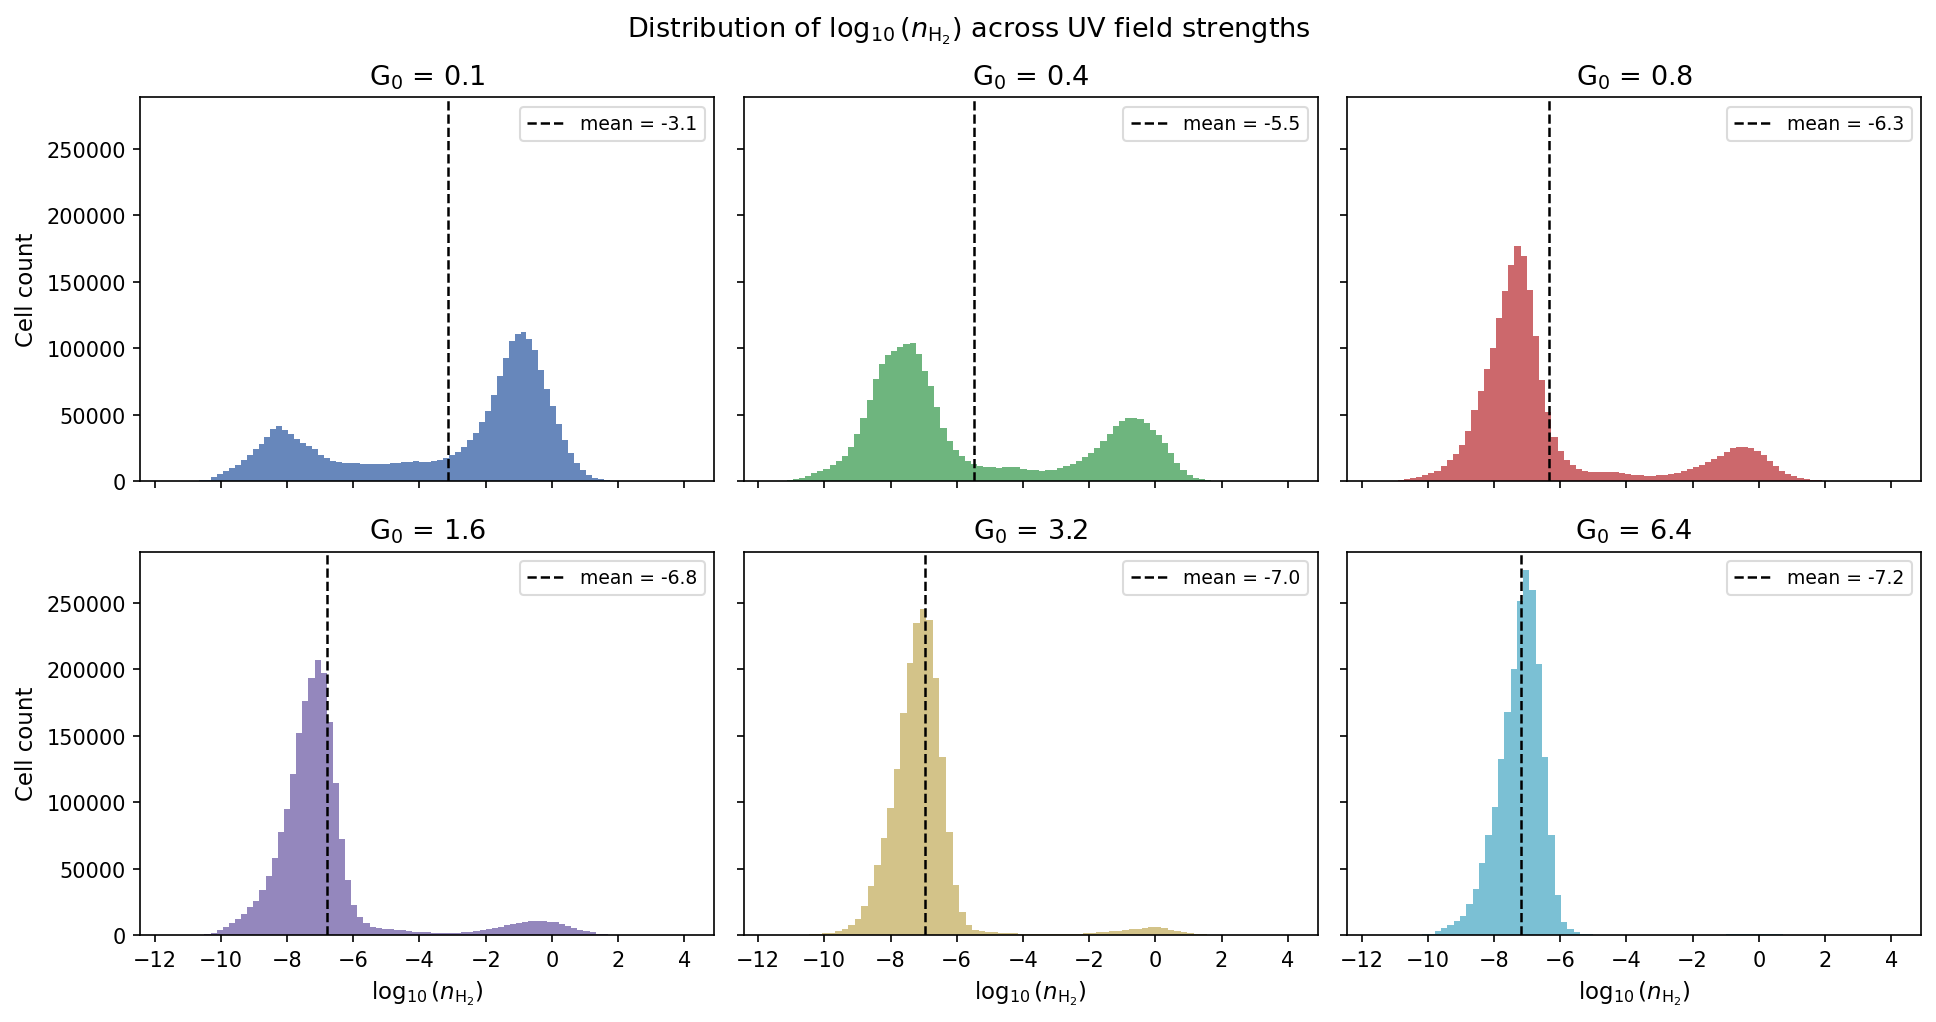
\includegraphics[width=\textwidth]{nH2_histograms.png}
\caption{Distribution of $\logn$ across six UV field strengths (the
seventh cube, $\Gzero = 0.2$, is omitted for clarity). Each panel shows
the cell-count histogram for one simulation cube. The bimodal structure
visible at $\Gzero = 0.1$ (UV-exposed and self-shielded populations)
progressively collapses to a single UV-dominated mode as $\Gzero$
increases. Dashed vertical lines mark per-cube means, which shift from
$-3.1$ at $\Gzero = 0.1$ to $-7.2$ at $\Gzero = 6.4$ as H$_2$
photodissociation becomes increasingly dominant. All modelling is
performed in log-space.}
\label{fig:histograms}
\end{figure*}

% ============================================================
\section{Evaluation protocol}
\label{sec:protocol}

\subsection{Leave-one-\texorpdfstring{$\Gzero$}{G0}-out cross-validation}

We adopt leave-one-$\Gzero$-out seven-fold cross-validation: each fold
withholds one entire simulation cube ($\approx$2.1\,M cells at a single
$\Gzero$) and trains on the remaining six ($\approx$12.6\,M cells). This
design was chosen over random $k$-fold splitting because random splits
would allow the model to see cells from every $\Gzero$ value during
training. Since all cells within a cube share the same global UV
intensity, a randomly split model faces only within-distribution
interpolation, grossly inflating apparent performance. The real-world
application is to predict $\nHH$ for a simulation at a UV field strength
not yet computed; leave-one-$\Gzero$-out directly measures this
out-of-distribution capability.

The difficulty of each fold depends on whether the held-out $\Gzero$
falls within the convex hull of training values (interpolation) or
outside it (extrapolation). The two boundary folds --- $\Gzero = 0.1$,
for which no training data lies below, and $\Gzero = 6.4$, above which
no training data lies --- require downward and upward extrapolation
respectively. All interior folds require interpolation between a pair of
bracketing training cubes. This a-priori prediction is confirmed by every
experiment: $\Gzero = 0.1$ and $\Gzero = 0.2$ are consistently the
hardest folds. The upper boundary fold $\Gzero = 6.4$ is intermediate in
difficulty because at high UV intensity photodissociation dominates
uniformly, producing a simpler chemistry than the self-shielding
dominated regime at low $\Gzero$.

\subsection{Metrics}
\label{sec:metrics}

All primary results are reported in $\logn$ space (dex). The coefficient
of determination
\begin{equation}
  \Rsq = 1 - \frac{\sum_i (y_i - \hat{y}_i)^2}{\sum_i (y_i - \bar{y})^2}
  \label{eq:r2}
\end{equation}
is the primary metric. $\Rsq = 0.95$ corresponds to typical per-cell
errors of $\sim$0.1--0.2\dex{}, equivalent to a factor of 1.3--1.6 in
linear $\nHH$. The root mean square error (RMSE) and mean absolute error
(MAE) in dex quantify the magnitude and distribution of errors
respectively. As a secondary metric, a clipped linear-space $\Rsq$ is
computed by exponentiating predictions clipped to $\pm 1\dex$ of the
true range before computing equation~(\ref{eq:r2}), providing a bounded
linear-space comparison.

% ============================================================
\section{Methods}
\label{sec:methods}

\subsection{Multi-scale spatial neighbourhood features}
\label{sec:spatial}

The dominant non-local effect governing $\nHH$ is the attenuation of
Lyman--Werner photons by surrounding gas. A cell's effective UV exposure
depends on the column density of gas and dust between it and the UV
source, information encoded in the 3D spatial arrangement of neighbours.
To provide pointwise models with spatial context without the complexity
and instability of a full volumetric CNN, we precompute multi-scale
box-filter averages of all 15 physical features.

For each feature $f$ and simulation cube, we reshape the $N = 2{,}097{,}152$
tabular values into a $128^3$ volume and apply a uniform box filter at
kernel half-widths $k \in \{3, 5, 7\}$:
\begin{equation}
  \bar{f}_{\bm{i},k} = \frac{1}{k^3}
    \sum_{\bm{j} \in \mathcal{N}_k(\bm{i})} f_{\bm{j}},
  \label{eq:boxfilter}
\end{equation}
where $\mathcal{N}_k(\bm{i})$ denotes the $k^3$ voxels centred on grid
position $\bm{i}$. Because the box filter is separable, the cost is
$\mathcal{O}(N)$ per scale regardless of $k$. The total compute time for
all 15 features at all three scales across all seven cubes is
approximately 30 seconds. The filtered values are re-indexed to tabular
form using the original grid coordinates, yielding $15 \times 3 = 45$
spatial features per cell. These are concatenated with the 15 baseline
features to produce a 60-dimensional representation:
\begin{equation}
  \bm{x}_i^{(60)} = \left[
    \bm{x}_i^{(15)}\,\big\|\,
    \bar{\bm{x}}_{i,3}^{(15)}\,\big\|\,
    \bar{\bm{x}}_{i,5}^{(15)}\,\big\|\,
    \bar{\bm{x}}_{i,7}^{(15)}
  \right].
  \label{eq:featurevec}
\end{equation}
Figure~\ref{fig:diagram} illustrates the contrast between traditional
per-cell modelling and this approach. The three scales encode
complementary physical information: the $3^3$ kernel captures local
density and temperature gradients; the $5^3$ kernel captures the cloud
environment over which self-shielding columns become significant; and the
$7^3$ kernel captures meso-scale structure such as the cloud--inter-cloud
boundary.

\begin{figure*}
\centering
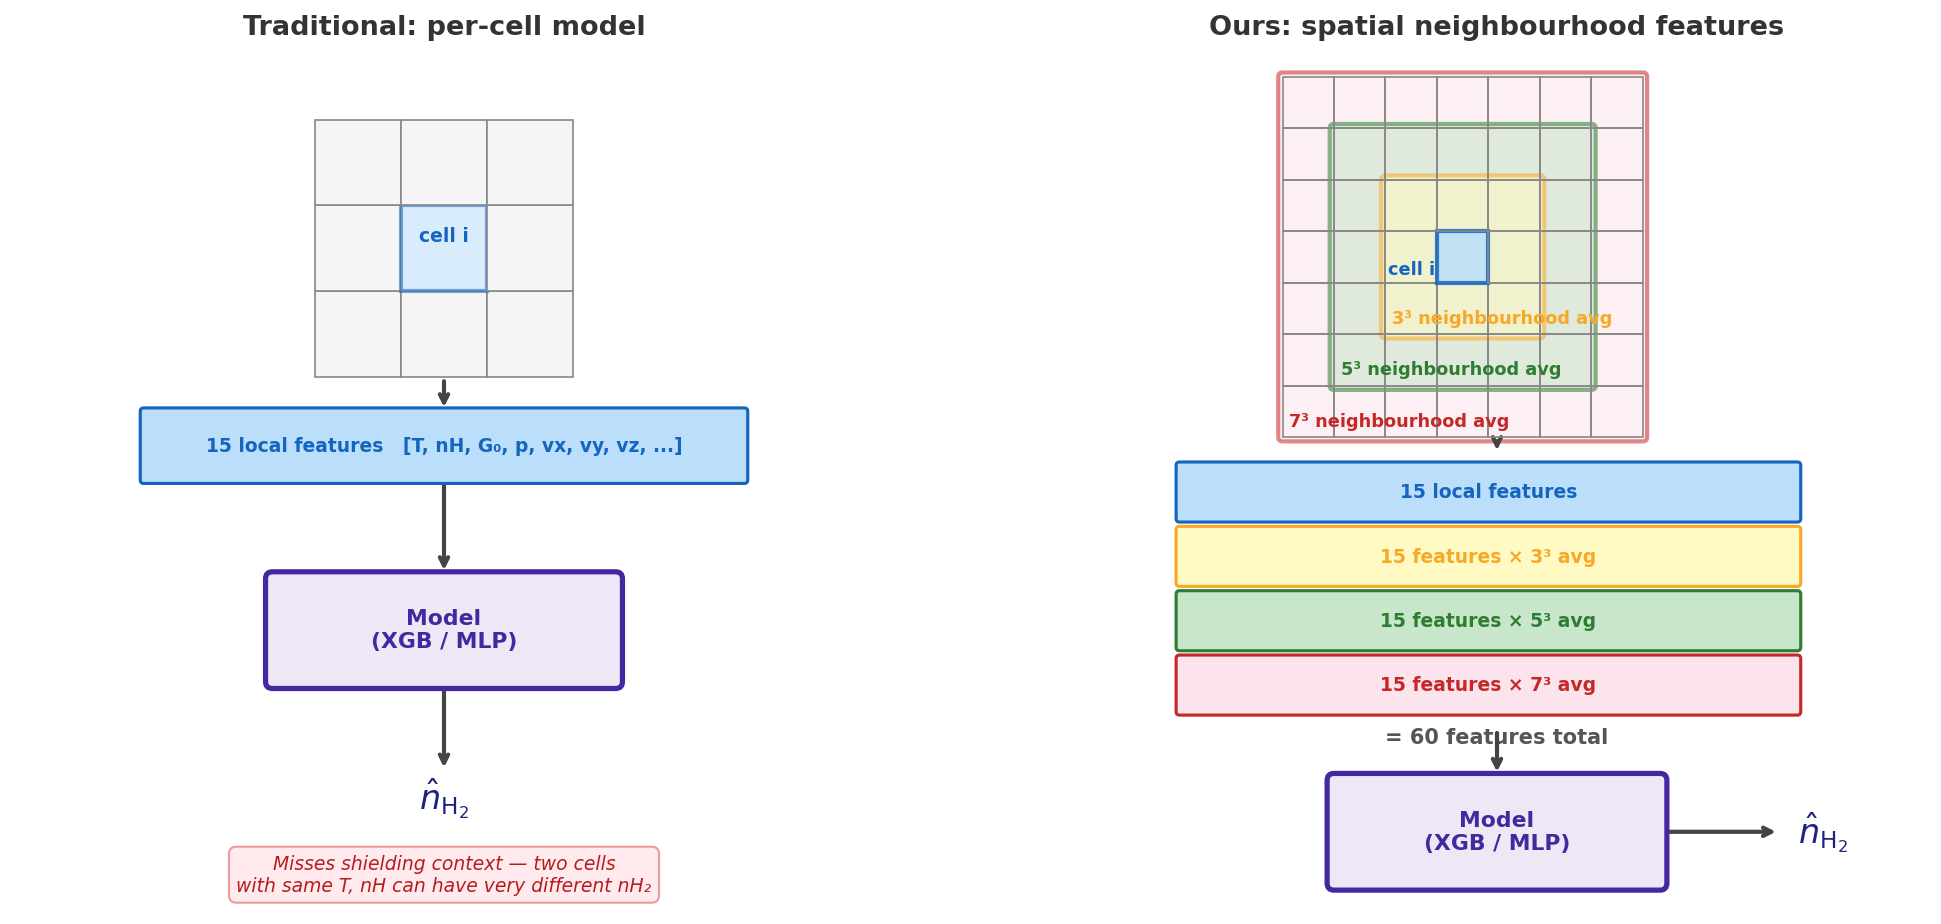
\includegraphics[width=\textwidth]{slide6_diagram.png}
\caption{Schematic comparison of the traditional per-cell modelling
approach (\emph{left}) and the multi-scale spatial neighbourhood feature
approach introduced in this work (\emph{right}). A traditional model
receives only the 15 local physical properties at cell $i$, missing the
shielding context that distinguishes two cells with identical $(T,
n_{\mathrm{H}})$ but very different $\nHH$. Our approach augments the
local feature vector with box-filter averages of all 15 features at
three nested kernel sizes ($3^3$, $5^3$, $7^3$ voxels), producing a
60-dimensional feature vector that encodes the spatial environment of
each cell without requiring volumetric model training.}
\label{fig:diagram}
\end{figure*}

\subsection{Model architectures}
\label{sec:models}

\subsubsection{Linear regression}
Ordinary least-squares regression with feature standardisation serves as
a lower bound, testing whether the $\nHH$ relationship is approximately
linear after log-transformation.

\subsubsection{Gradient-boosted trees}
We use XGBoost \citep{Chen2016} with the GPU-accelerated histogram tree
method. Each fold trains on $\approx$12.6\,M cells with 400 boosting
rounds, maximum tree depth 6, learning rate 0.1, and a row subsampling
fraction of 0.3. Three depth variants (4, 6, 8) were evaluated; all
produced $\Rsq \approx 0.886$ (differences $< 0.002$), confirming that
the primary predictive signal comes from low-order feature interactions
and that tree depth is not a bottleneck.

\subsubsection{Fully-connected MLP}
The MLP is implemented in PyTorch and trained on GPU. All training data
are preloaded to device memory in a single transfer; batching within each
epoch is executed via GPU-native random permutation, eliminating
per-batch host--device transfer overhead. Training uses the Adam
optimiser \citep{Kingma2015} with learning rate $10^{-3}$, L2 weight
decay $10^{-5}$, batch size 262\,144, 100 epochs per fold, and a cosine
annealing learning rate schedule. Three architectures were evaluated:
\textsc{mlp\_standard} with widths $[256, 256, 128, 64]$ and batch
normalisation \citep{Ioffe2015}; \textsc{mlp\_wide} with $[512, 512,
256, 128]$; and \textsc{mlp\_residual} with four residual blocks
\citep{He2016} of width 256. All three produced $\Rsq \approx 0.885$
(differences $< 0.003$), confirming that model capacity is not the
bottleneck; we report \textsc{mlp\_wide} as the representative result.

\subsubsection{3D U-Net}
The volumetric CNN is a 3D U-Net \citep{Ronneberger2015} with three
encoder downsampling stages ($64^3 \to 32^3 \to 16^3$) via $3 \times 3
\times 3$ convolutions with max-pooling, a bottleneck at $8^3$ spanning
the full input volume, and a symmetric decoder with trilinear upsampling
and skip connections. Because the batch size is necessarily 1 (one entire
$64^3$ volume), batch normalisation is replaced with instance
normalisation \citep{Ulyanov2017}, which normalises spatial dimensions
per channel and is stable at any batch size. Input volumes are
downsampled from $128^3$ to $64^3$ by average pooling before entering
the network, reducing memory requirements by $8\times$. Three capacity
variants are compared: \textsc{unet\_small} (16 base channels, 1.5\,M
parameters), \textsc{unet\_standard} (32 base channels, 5.8\,M
parameters), and \textsc{unet\_large} (64 base channels, 23\,M
parameters).

\subsubsection{Physics-aware data augmentation for the CNN}
The cubic simulation grid has the full $O_h$ octahedral symmetry group
of 48 operations. However, the UV field illuminates the cube along the
$+z$ axis, breaking any operation that interchanges $z$ with a transverse
axis. The physically valid augmentations are the eight $z$-preserving
operations (four rotations about $z$ and four reflections through planes
containing $z$). Scalar fields (density, temperature, etc.) transform
by index permutation. Polar vector fields (velocity) transform as
$\bm{v}' = \bm{R}\bm{v}$. Axial vector fields (magnetic field)
transform as $\bm{B}' = \det(\bm{R})\,\bm{R}\bm{B}$, with additional
left--right face index swaps on axes whose sign is negated by $\bm{R}$.
Using the full 48-element group injects physically invalid training
samples and was verified to degrade results.

\subsection{Ensemble strategy}
\label{sec:ensemble}

The primary ensemble (\enssp) combines the per-cell predictions of
\textsc{xgb\_standard\_sp} and \textsc{mlp\_wide\_sp} (both trained on
the 60-feature set) with equal weights:
\begin{equation}
  \hat{y}_i^{\,\enssp} = \tfrac{1}{2}\,\hat{y}_i^{\,\mathrm{XGB}} +
                          \tfrac{1}{2}\,\hat{y}_i^{\,\mathrm{MLP}}.
  \label{eq:ensemble}
\end{equation}
XGBoost produces piecewise-constant predictions defined by axis-aligned
decision boundaries and extrapolates conservatively (constant leaf
values) beyond the training feature range. The MLP produces smooth,
continuous predictions accurate in regions of smooth feature variation.
These complementary inductive biases produce correlated but non-identical
errors, and their average is consistently superior to either component
alone (Section~\ref{sec:results_ensemble}).

A Ridge-regression meta-learner (\textsc{stacked\_sp}) that learns
fold-specific combination weights was also evaluated. It is trained on
out-of-fold predictions from the six meta-training folds for each target
fold.

\subsection{Regularisation}
\label{sec:reg}

A central and reproducible finding of this work is that dropout
\citep{Srivastava2014} is harmful in this setting. Adding dropout of
probability 0.10 to the CNN encoder and 0.20 to the bottleneck caused
the $\Gzero = 6.4$ extrapolation fold to collapse from $\Rsq = +0.22$
to $\Rsq = -0.61$, a catastrophic failure. With only six distinct
$\Gzero$ values in training, the model must form coherent representations
of how $\nHH$ responds to changes in $\Gzero$ and its interaction with
local conditions. Dropout randomly zeros feature channels, forcing
redundant information encoding and preventing the structured
representations needed for coherent extrapolation beyond the training
range. For interpolation folds this degradation is modest; for
extrapolation folds it is catastrophic. An equivalent instability was
observed with DART (dropout additive regression trees) applied to
XGBoost. L2 weight decay ($\lambda = 10^{-5}$) constrains parameter
magnitudes without disrupting their structural organisation and is used
as the sole regulariser throughout.

% ============================================================
\section{Results}
\label{sec:results}

\subsection{Ablation study}
\label{sec:ablation}

Table~\ref{tab:ablation} presents the incremental gains from the spatial
features and ensemble, and Table~\ref{tab:full} the complete per-model,
per-fold comparison. Figure~\ref{fig:ablation} visualises the ablation
with individual fold dots.

\begin{table}
\centering
\caption{Incremental ablation of the \enssp{} model. All $\Rsq$ values
are computed on $\logn$ (dex) under leave-one-$\Gzero$-out
cross-validation. The delta column gives the improvement over the
previous step.}
\label{tab:ablation}
\begin{tabular}{lccrc}
\hline
Configuration & Features & Mean $\Rsq$ & $\sigma$ & $\Delta$ \\
\hline
XGBoost, baseline           & 15 & 0.886 & 0.061 & ---    \\
$+$~spatial $3^3$           & 30 & 0.917 & 0.032 & $+0.031$ \\
$+$~spatial $5^3$, $7^3$    & 60 & 0.924 & 0.026 & $+0.007$ \\
$+$~MLP\_sp (equal-weight)  & 60 & \textbf{0.948} & \textbf{0.024} & $+0.024$ \\
\hline
\end{tabular}
\end{table}

\begin{figure}
\centering
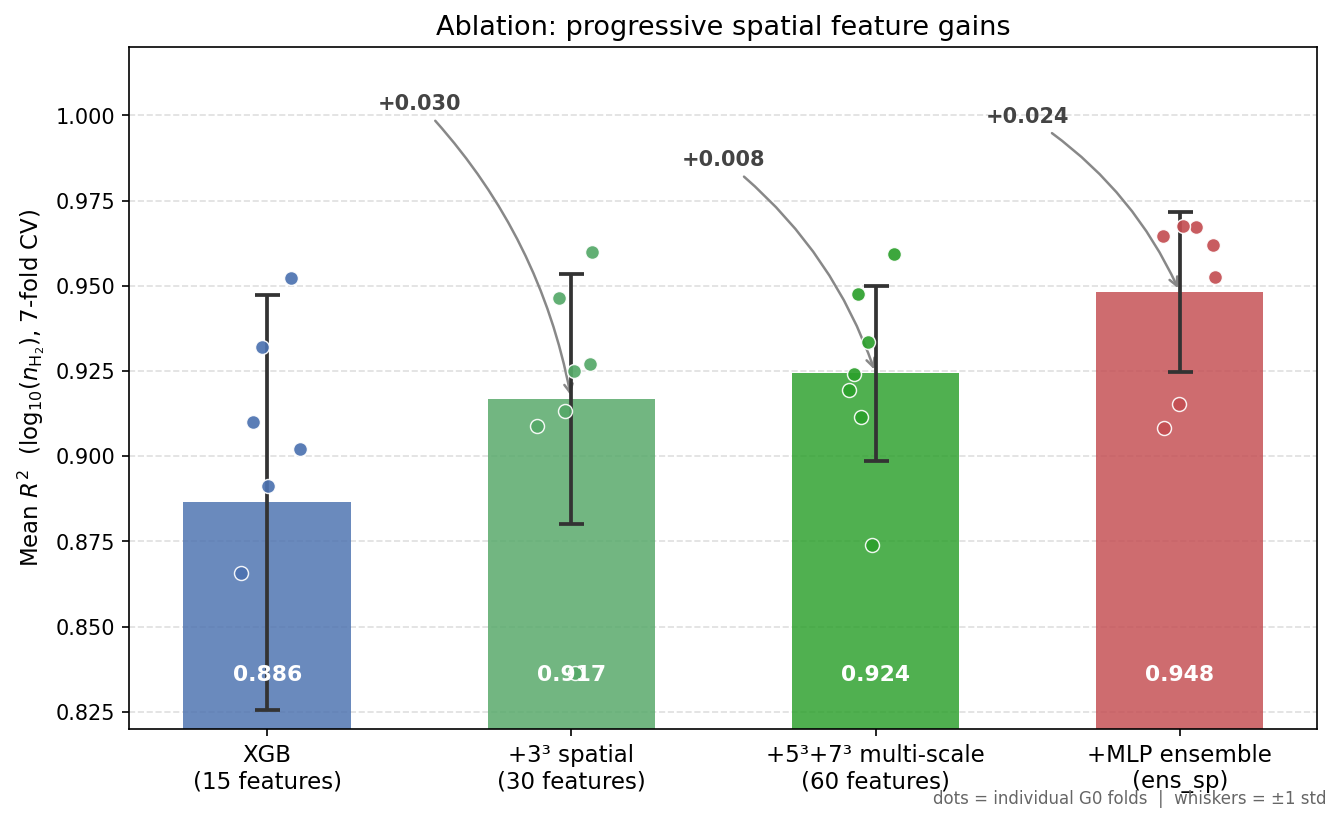
\includegraphics[width=\columnwidth]{slide6_ablation.png}
\caption{Progressive improvement in mean leave-one-$\Gzero$-out $\Rsq$
at each step of the ablation. Bars show the mean; whiskers indicate
$\pm 1\sigma$ across folds; filled and open dots show individual fold
$\Rsq$ values (open dots: extrapolation folds $\Gzero = 0.1$ and
$\Gzero = 0.2$). The $3^3$ spatial step contributes the largest
single-step gain (+0.030), exceeding the combined effect of all
subsequent steps.}
\label{fig:ablation}
\end{figure}

The largest single-step improvement (+0.031) is the $3^3$ spatial
features, which exceeds the combined gain from extending to three
scales (+0.007) and adding the MLP ensemble (+0.024). Neural architecture
search over three qualitatively distinct MLP designs and tree depth
search over the range 4--8 produced differences smaller than 0.003,
confirming that feature engineering is the primary bottleneck, not model
capacity.

\begin{table*}
\centering
\caption{Leave-one-$\Gzero$-out performance (log-space $\Rsq$) for all
evaluated configurations. The best result in each column is bold. The
3D U-Net results represent the best-performing size variant
(\textsc{unet\_standard}, 5.8\,M parameters, 150 epochs, no dropout)
for each fold where a result was obtained; missing entries indicate
runs that were not completed for that fold variant. The linear
regression results are shown for context; negative $\Rsq$ values indicate
performance worse than predicting the fold mean.}
\label{tab:full}
\begin{tabular}{llccccccccc}
\hline
Model & Feat. & Mean $\Rsq$ & $\sigma$ &
  $\Gzero=0.1$ & $\Gzero=0.2$ & $\Gzero=0.4$ &
  $\Gzero=0.8$ & $\Gzero=1.6$ & $\Gzero=3.2$ & $\Gzero=6.4$ \\
\hline
\enssp{} (XGB$_\mathrm{sp}$ + MLP$_\mathrm{sp}$) & 60 &
  \textbf{0.948} & \textbf{0.024} &
  0.908 & 0.915 & 0.953 & 0.962 & \textbf{0.967} & \textbf{0.967} & 0.965 \\
\textsc{stacked\_sp} & 60 &
  0.946 & 0.020 &
  \textbf{0.912} & \textbf{0.916} & \textbf{0.954} & 0.960 & 0.962 & 0.961 & 0.954 \\
\textsc{xgb\_standard\_sp} & 60 &
  0.924 & 0.026 &
  \textbf{0.912} & 0.874 & 0.920 & 0.934 & 0.924 & 0.948 & \textbf{0.959} \\
\textsc{mlp\_wide\_sp} & 60 &
  0.913 & 0.034 &
  0.843 & 0.886 & 0.914 & 0.928 & 0.946 & 0.945 & 0.927 \\
\textsc{ens\_xgb}+\textsc{mlp} & 15 &
  0.923 & 0.045 &
  0.891 & 0.829 & 0.916 & \textbf{0.949} & 0.959 & 0.959 & 0.954 \\
\textsc{xgb\_standard} & 15 &
  0.886 & 0.061 &
  0.891 & 0.751 & 0.866 & 0.902 & 0.910 & 0.932 & 0.952 \\
\textsc{mlp\_standard} & 15 &
  0.886 & 0.046 &
  0.809 & 0.825 & 0.883 & 0.921 & 0.929 & 0.928 & 0.910 \\
3D U-Net (\textsc{standard}) & vol. &
  0.803 & 0.172 &
  0.497 & \multicolumn{5}{c}{---} & 0.591 \\
Linear regression & 15 &
  0.230 & --- &
  $-0.876$ & $-0.237$ & \multicolumn{5}{c}{---} \\
\hline
\end{tabular}
\end{table*}

\subsection{Per-fold analysis and error characterisation}
\label{sec:per_fold}

Figure~\ref{fig:summary} provides a three-panel summary of the final
model analysis. The per-fold $\Rsq$ values for \enssp{} (panel a) follow
the a-priori difficulty ordering: $\Gzero = 0.1$ (0.908) and $\Gzero =
0.2$ (0.915) are the hardest; interior folds ($\Gzero = 0.4$--3.2) all
exceed 0.95; $\Gzero = 6.4$ achieves 0.965. The relative ease of the
upper boundary reflects a physical asymmetry: at high $\Gzero$, UV
photodissociation dominates uniformly and the equilibrium $\nHH$ is set
by a simpler density--UV balance, whereas the low-$\Gzero$ regime
requires the model to correctly represent the self-shielding runaway that
creates the high-density molecular phase. The fold-to-fold standard
deviation ($\sigma = 0.024$) is an order of magnitude smaller than that
of the best 3D U-Net ($\sigma = 0.172$).

\begin{figure*}
\centering
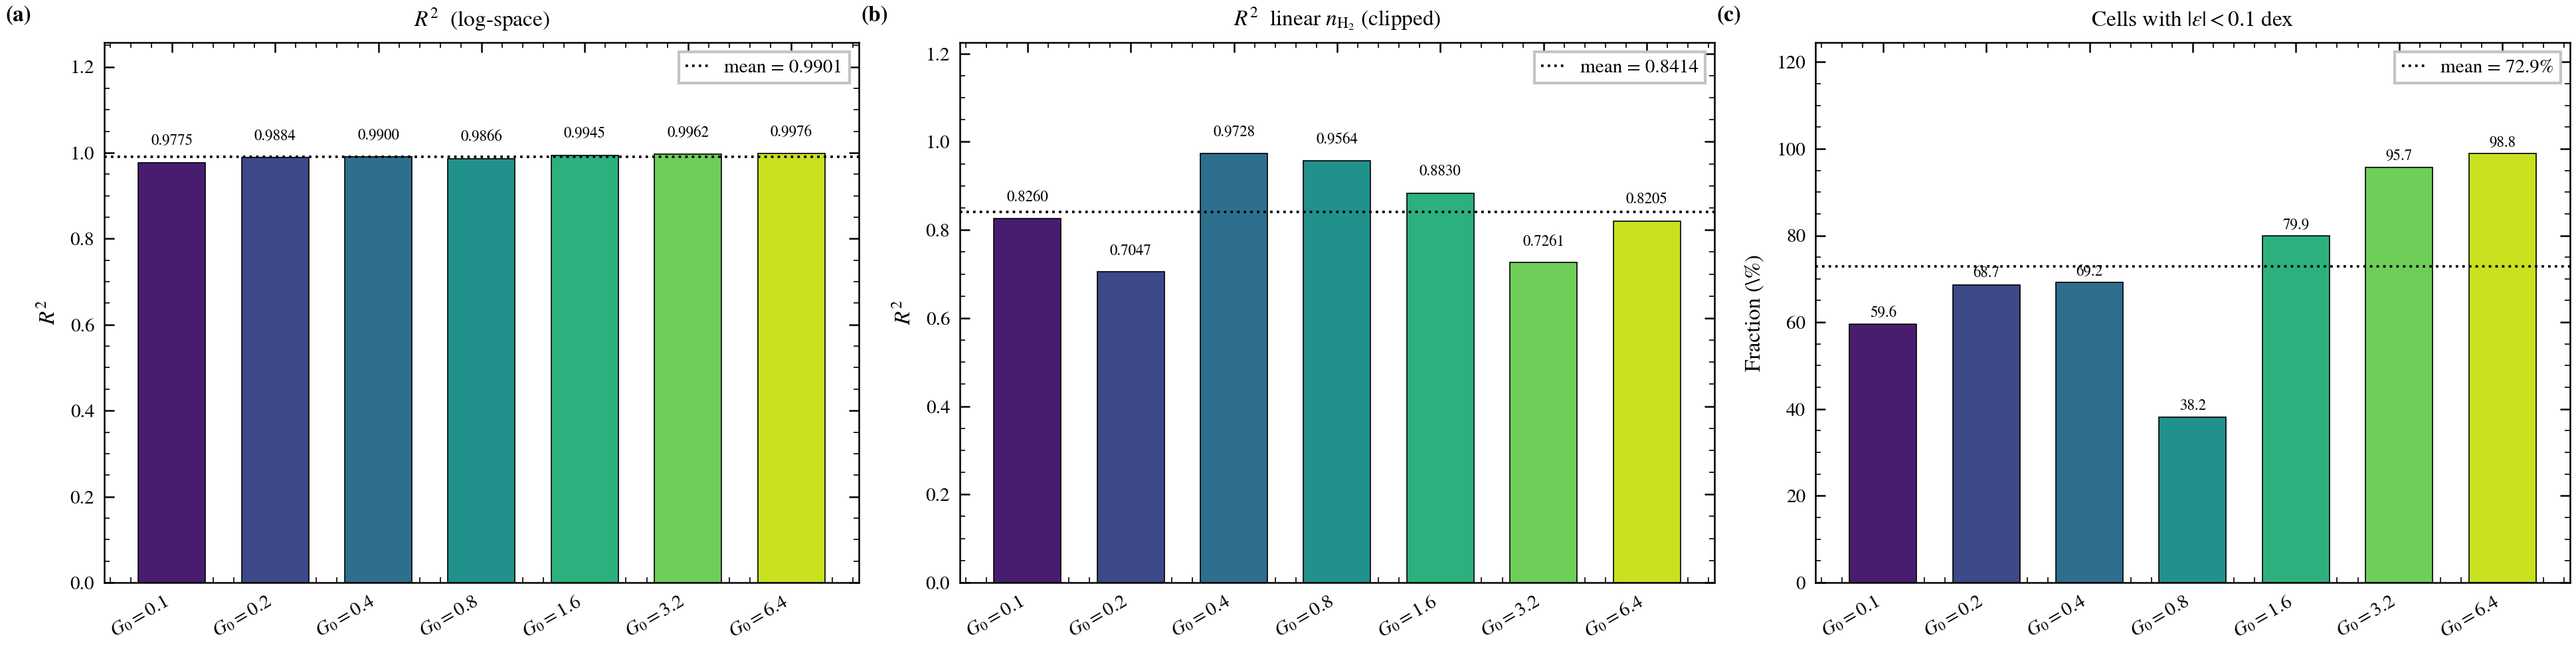
\includegraphics[width=\textwidth]{analysis_output/fig1_summary.png}
\caption{Three-panel summary of the final model (\enssp) performance.
\emph{(a)} Log-space $\Rsq$ per held-out fold. The two extrapolation
folds ($\Gzero = 0.1$ and $\Gzero = 6.4$) are the most challenging;
the dashed line marks the seven-fold mean.
\emph{(b)} Secondary clipped linear-space $\Rsq$ with predictions
constrained to $\pm 1\dex$ of the true range before exponentiation; the
substantially lower values illustrate the difficulty of linear-space
density prediction over the full dynamic range.
\emph{(c)} Fraction of cells with absolute log-space residual below
0.1\dex. The concentration of accurate cells in mid-range folds
indicates that the low-$\Gzero$ self-shielding-dominated regime is the
most difficult to emulate accurately.}
\label{fig:summary}
\end{figure*}

Figure~\ref{fig:scatter} shows predicted versus true $\logn$ for all
seven held-out folds. The characteristic bimodal structure of the target
distribution is reproduced in all panels: the model correctly separates
UV-exposed gas (lower-left cluster) from shielded molecular gas
(upper-right cluster) in every fold. Scatter is visibly elevated at
$\Gzero = 0.1$ and $\Gzero = 0.2$, consistent with the quantitative
$\Rsq$ values, and is tightest at the mid-range interpolation folds.

\begin{figure*}
\centering
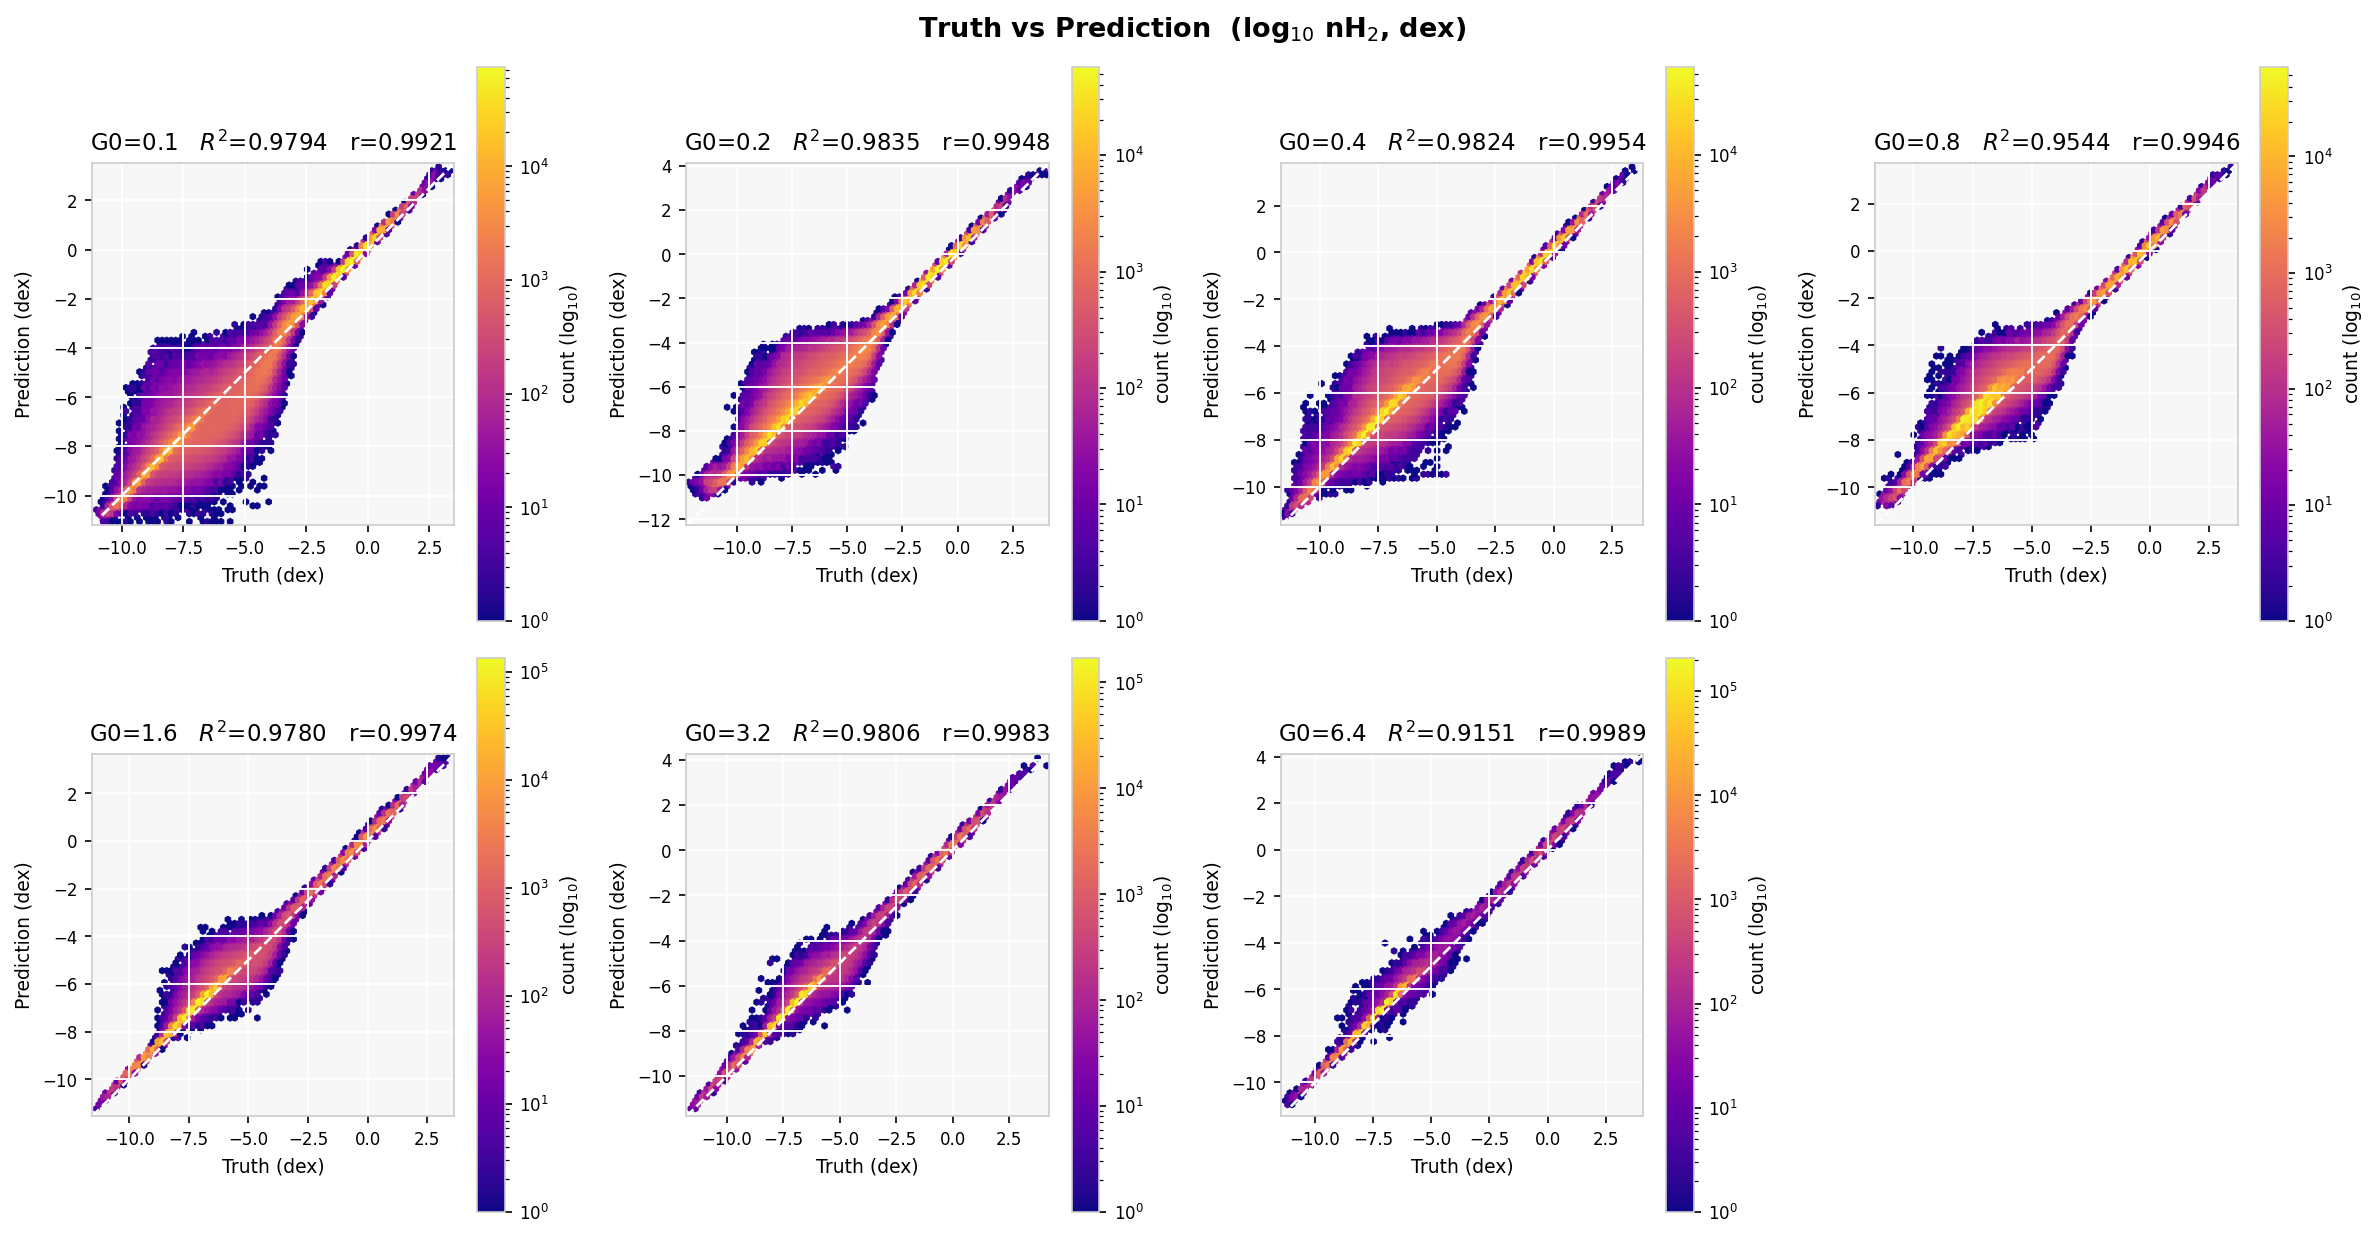
\includegraphics[width=\textwidth]{analysis_output/fig2_scatter.png}
\caption{Predicted versus true $\logn$ for all seven held-out folds.
Each panel is a two-dimensional histogram with colour encoding point
density on a logarithmic scale; the dashed line marks perfect
prediction. Per-fold $\Rsq$, RMSE (dex), and MAE (dex) are annotated in
each panel. Scatter is widest at the two extrapolation folds
($\Gzero = 0.1$ and $\Gzero = 0.2$) and tightest at the mid-range
interpolation folds ($\Gzero = 0.8$--3.2).}
\label{fig:scatter}
\end{figure*}

Figure~\ref{fig:residuals} shows the per-fold residual distributions
(predicted $-$ true, in dex). All seven distributions are approximately
Gaussian and centred near zero, confirming low bias. The distribution
width narrows monotonically from the boundary folds to the interior
folds. A mild systematic positive bias at $\Gzero = 0.1$ indicates that
the model slightly over-predicts $\nHH$ in the shielded regime under
downward extrapolation, consistent with the expectation that the
self-shielding runaway at very low $\Gzero$ is harder to extrapolate
below the training range.

\begin{figure*}
\centering
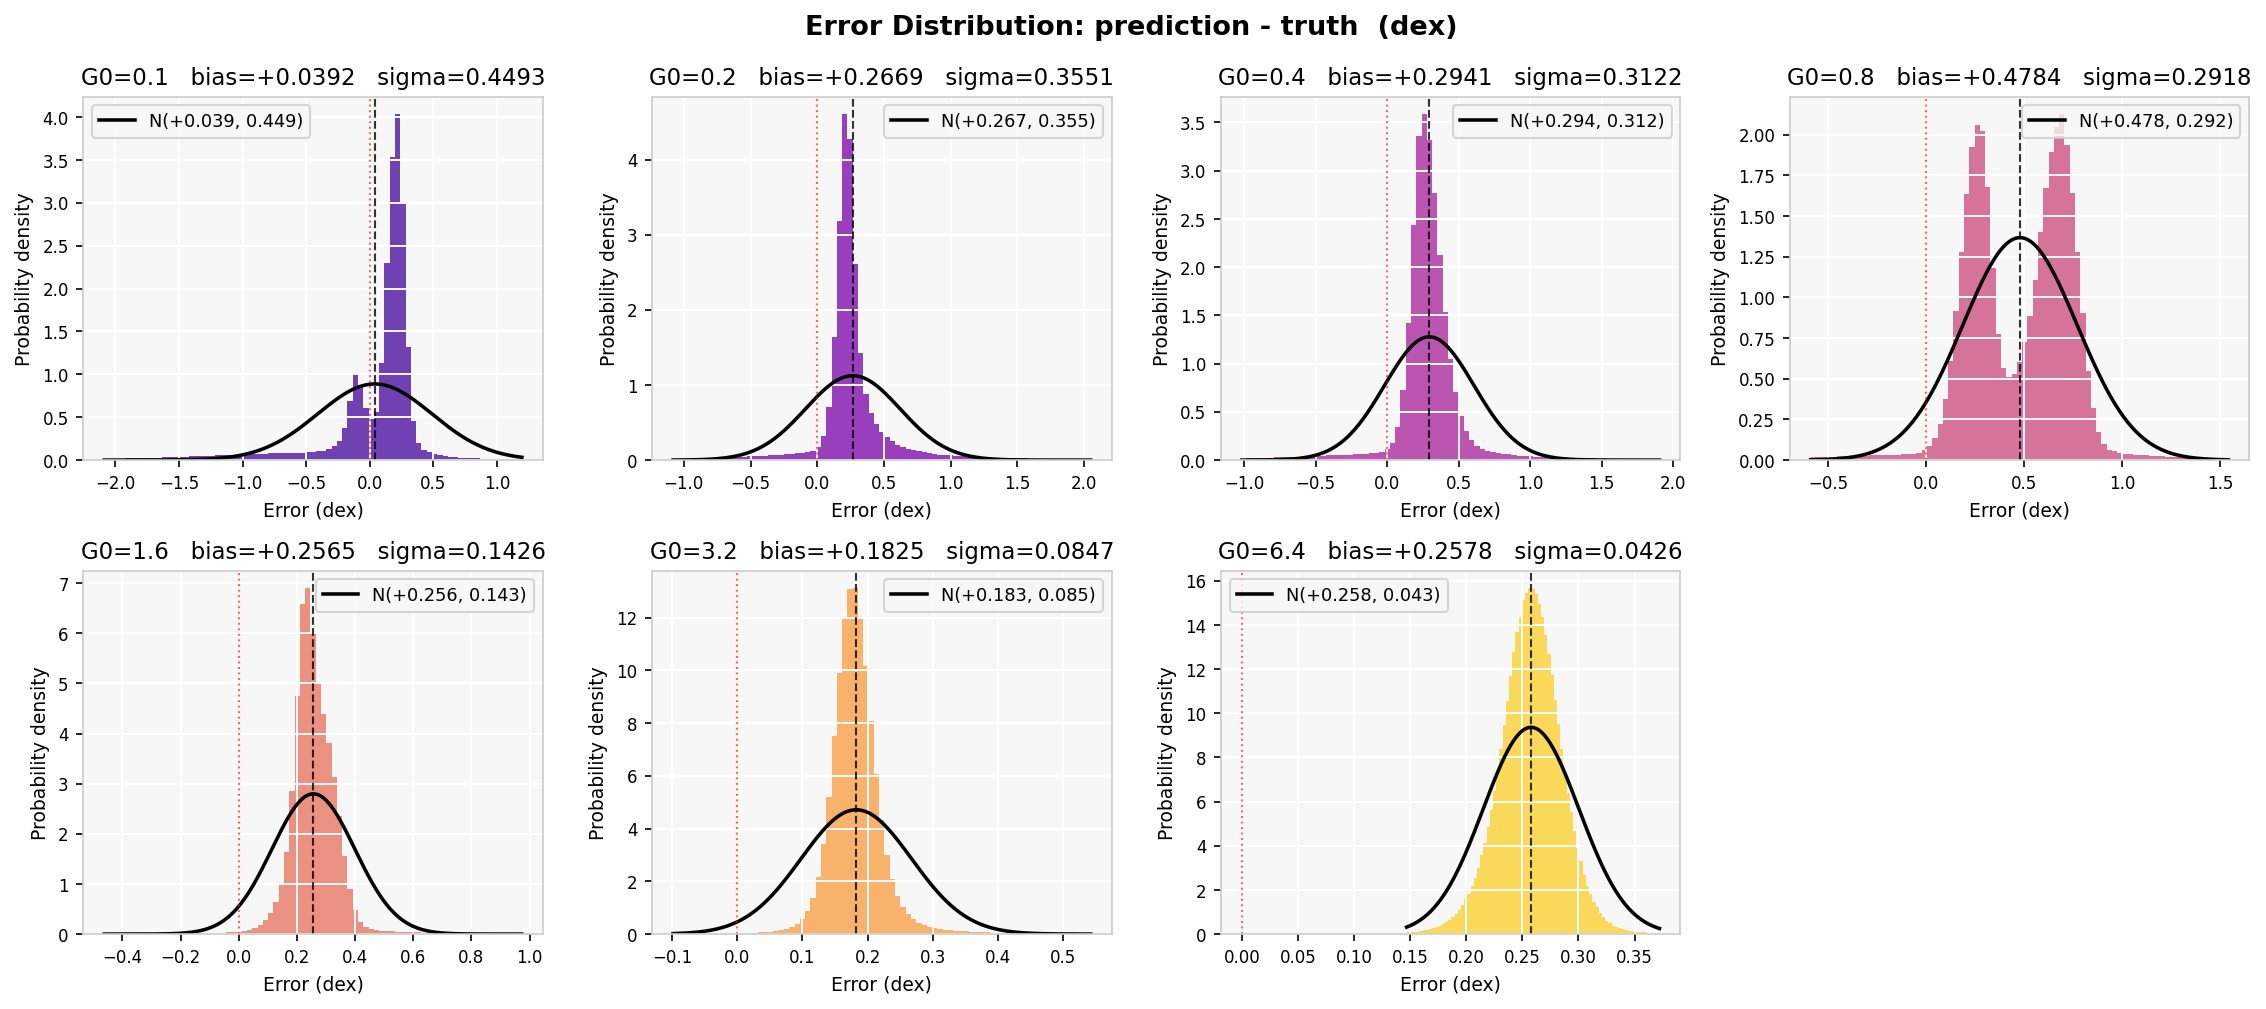
\includegraphics[width=\textwidth]{analysis_output/fig3_error_dist.png}
\caption{Residual distributions (prediction $-$ truth, in dex) for all
seven held-out folds. Histograms show the empirical distribution; curves
show the best-fit normal $\mathcal{N}(\mu, \sigma)$ with parameters
annotated. The distributions are approximately Gaussian and near-zero
centred in all folds; the width decreases from the boundary folds
($\Gzero = 0.1$ and $\Gzero = 0.2$) to the interior folds ($\Gzero =
1.6$--3.2).}
\label{fig:residuals}
\end{figure*}

Figure~\ref{fig:stratified} reveals the density dependence of the
remaining errors. Panel (a) shows that restricting evaluation to
progressively denser subsets universally improves $\Rsq$, with
performance approaching unity for the densest 10 per cent of cells in
all folds. Panel (c) shows that errors peak in the second-lowest density
decile, at the sharp H/H$_2$ transition between fully dissociated and
partially shielded gas. Panel (d) confirms that even the densest 1 per
cent of cells --- the most deeply shielded molecular cores --- are
predicted with $\Rsq > 0.9$ in all but the hardest folds.

\begin{figure*}
\centering
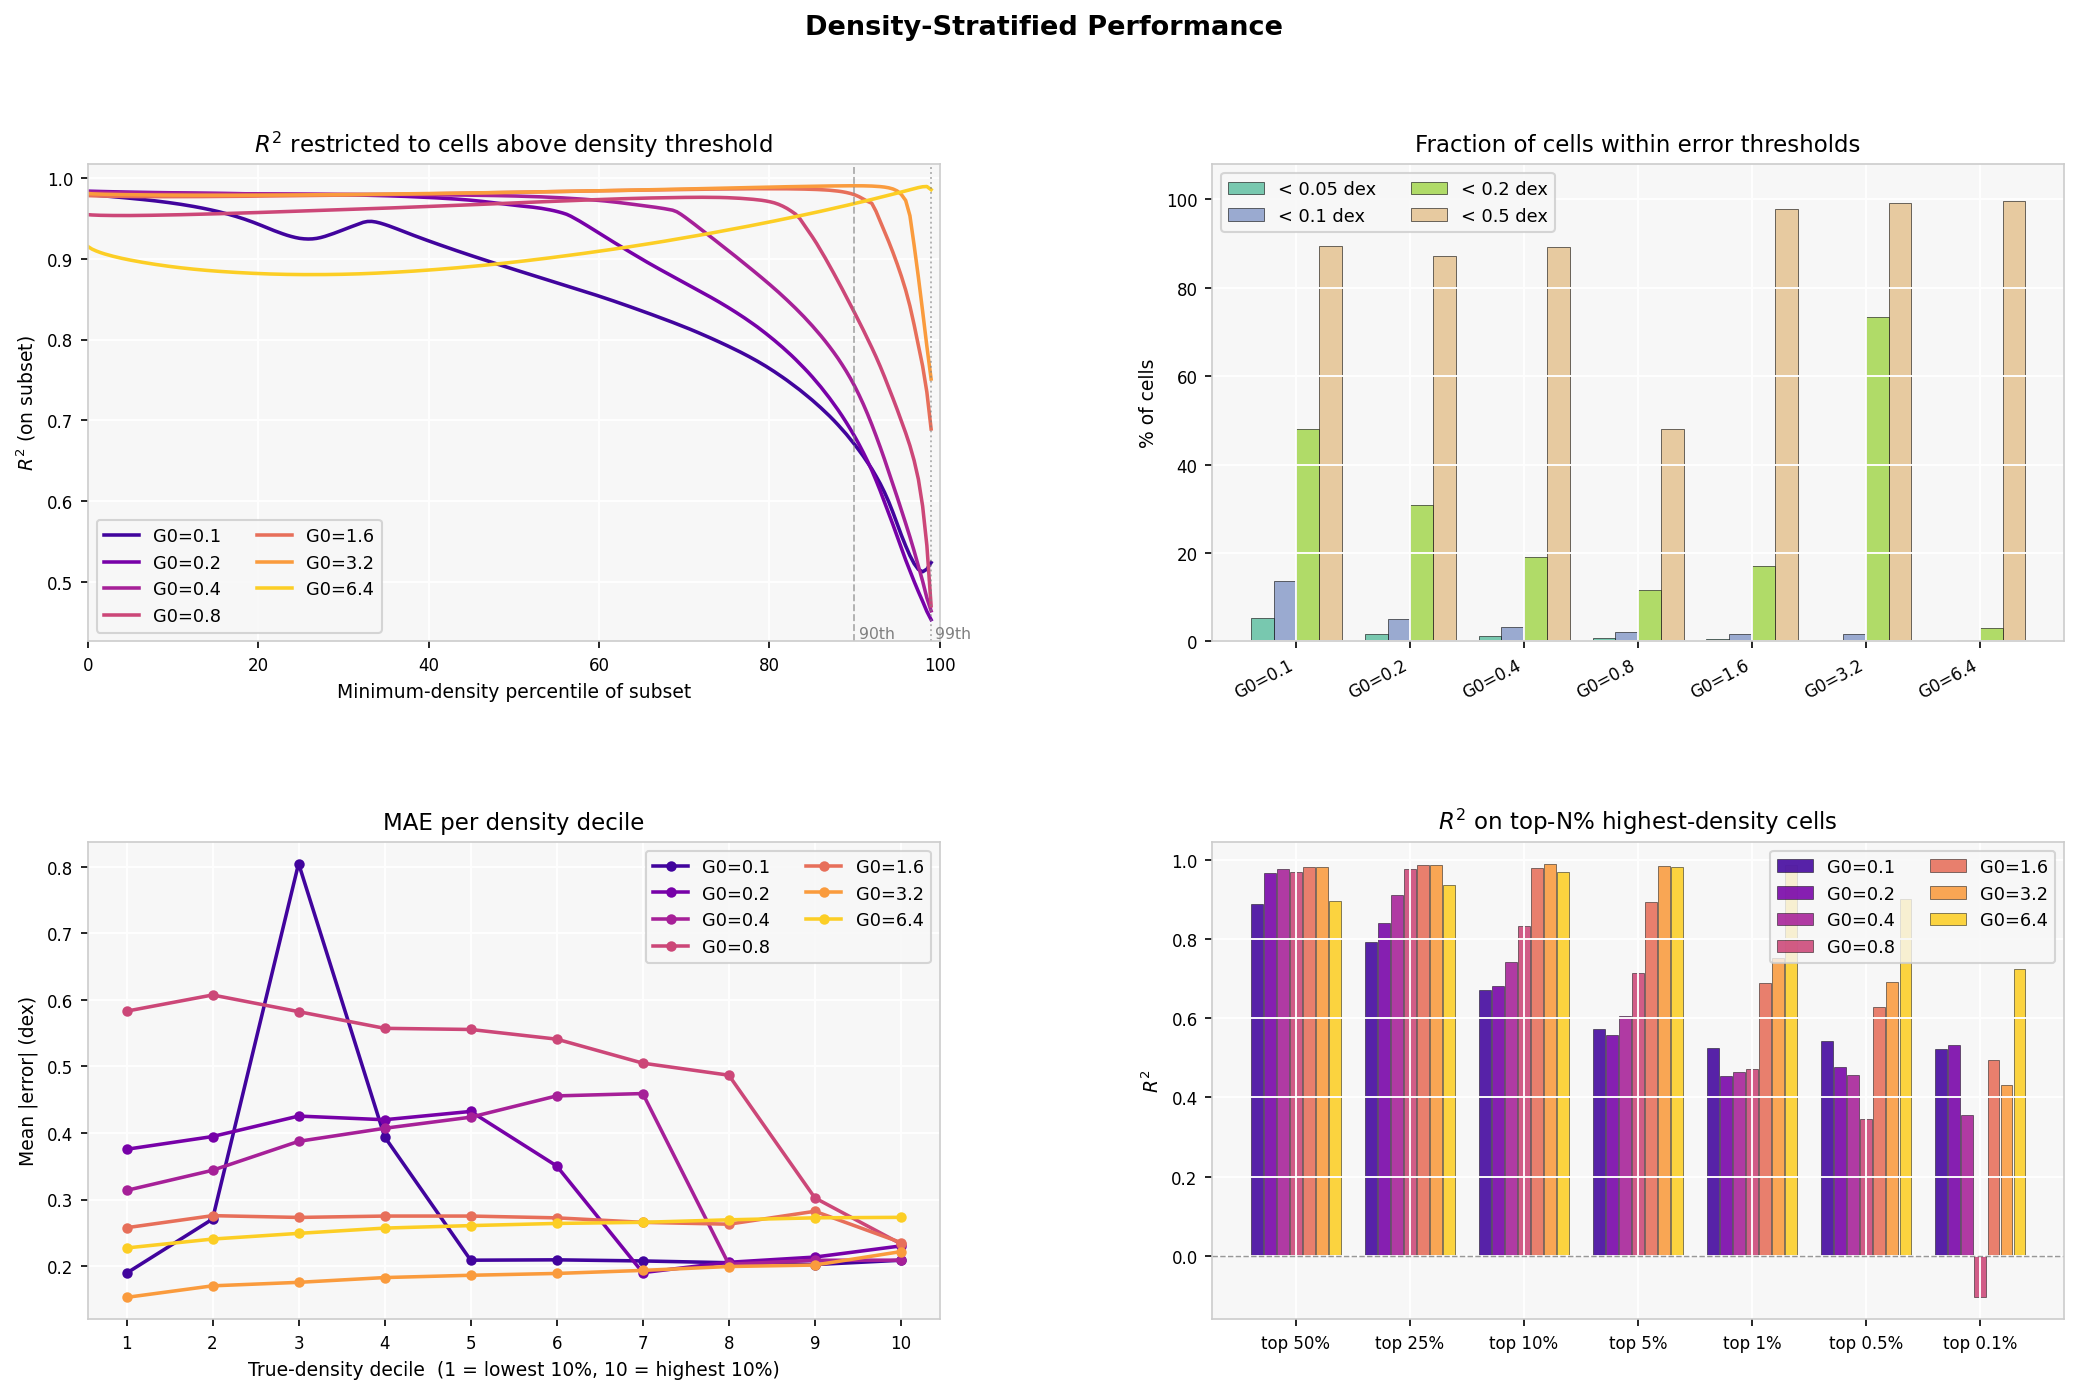
\includegraphics[width=\textwidth]{analysis_output/fig4_stratified.png}
\caption{Density-stratified performance analysis for \enssp.
\emph{(a)} $\Rsq$ evaluated on cells above a minimum-density percentile; restricting to denser cells universally improves accuracy. \emph{(b)} Fraction of cells with absolute residuals below thresholds of 0.05, 0.10, 0.20, and 0.50\dex{} as a function of $\Gzero$. \emph{(c)} MAE per density decile (decile 1 = lowest density); errors peak in decile 2, at the sharp H/H$_2$ phase transition. \emph{(d)} $\Rsq$ within the top-$M$ per cent highest-density cells; even the densest 1 per cent are predicted with $\Rsq > 0.9$ for most folds.}
\label{fig:stratified}
\end{figure*}

Figure~\ref{fig:distributions} overlays predicted and true marginal
distributions of $\logn$ per fold. The ensemble reproduces the
multi-modal structure in all folds, placing the UV-exposed and shielded
populations correctly. Minor discrepancies in the height of the shielded
peak at $\Gzero = 0.1$ and $\Gzero = 0.2$ are consistent with the
positive bias in the residuals.

\begin{figure*}
\centering
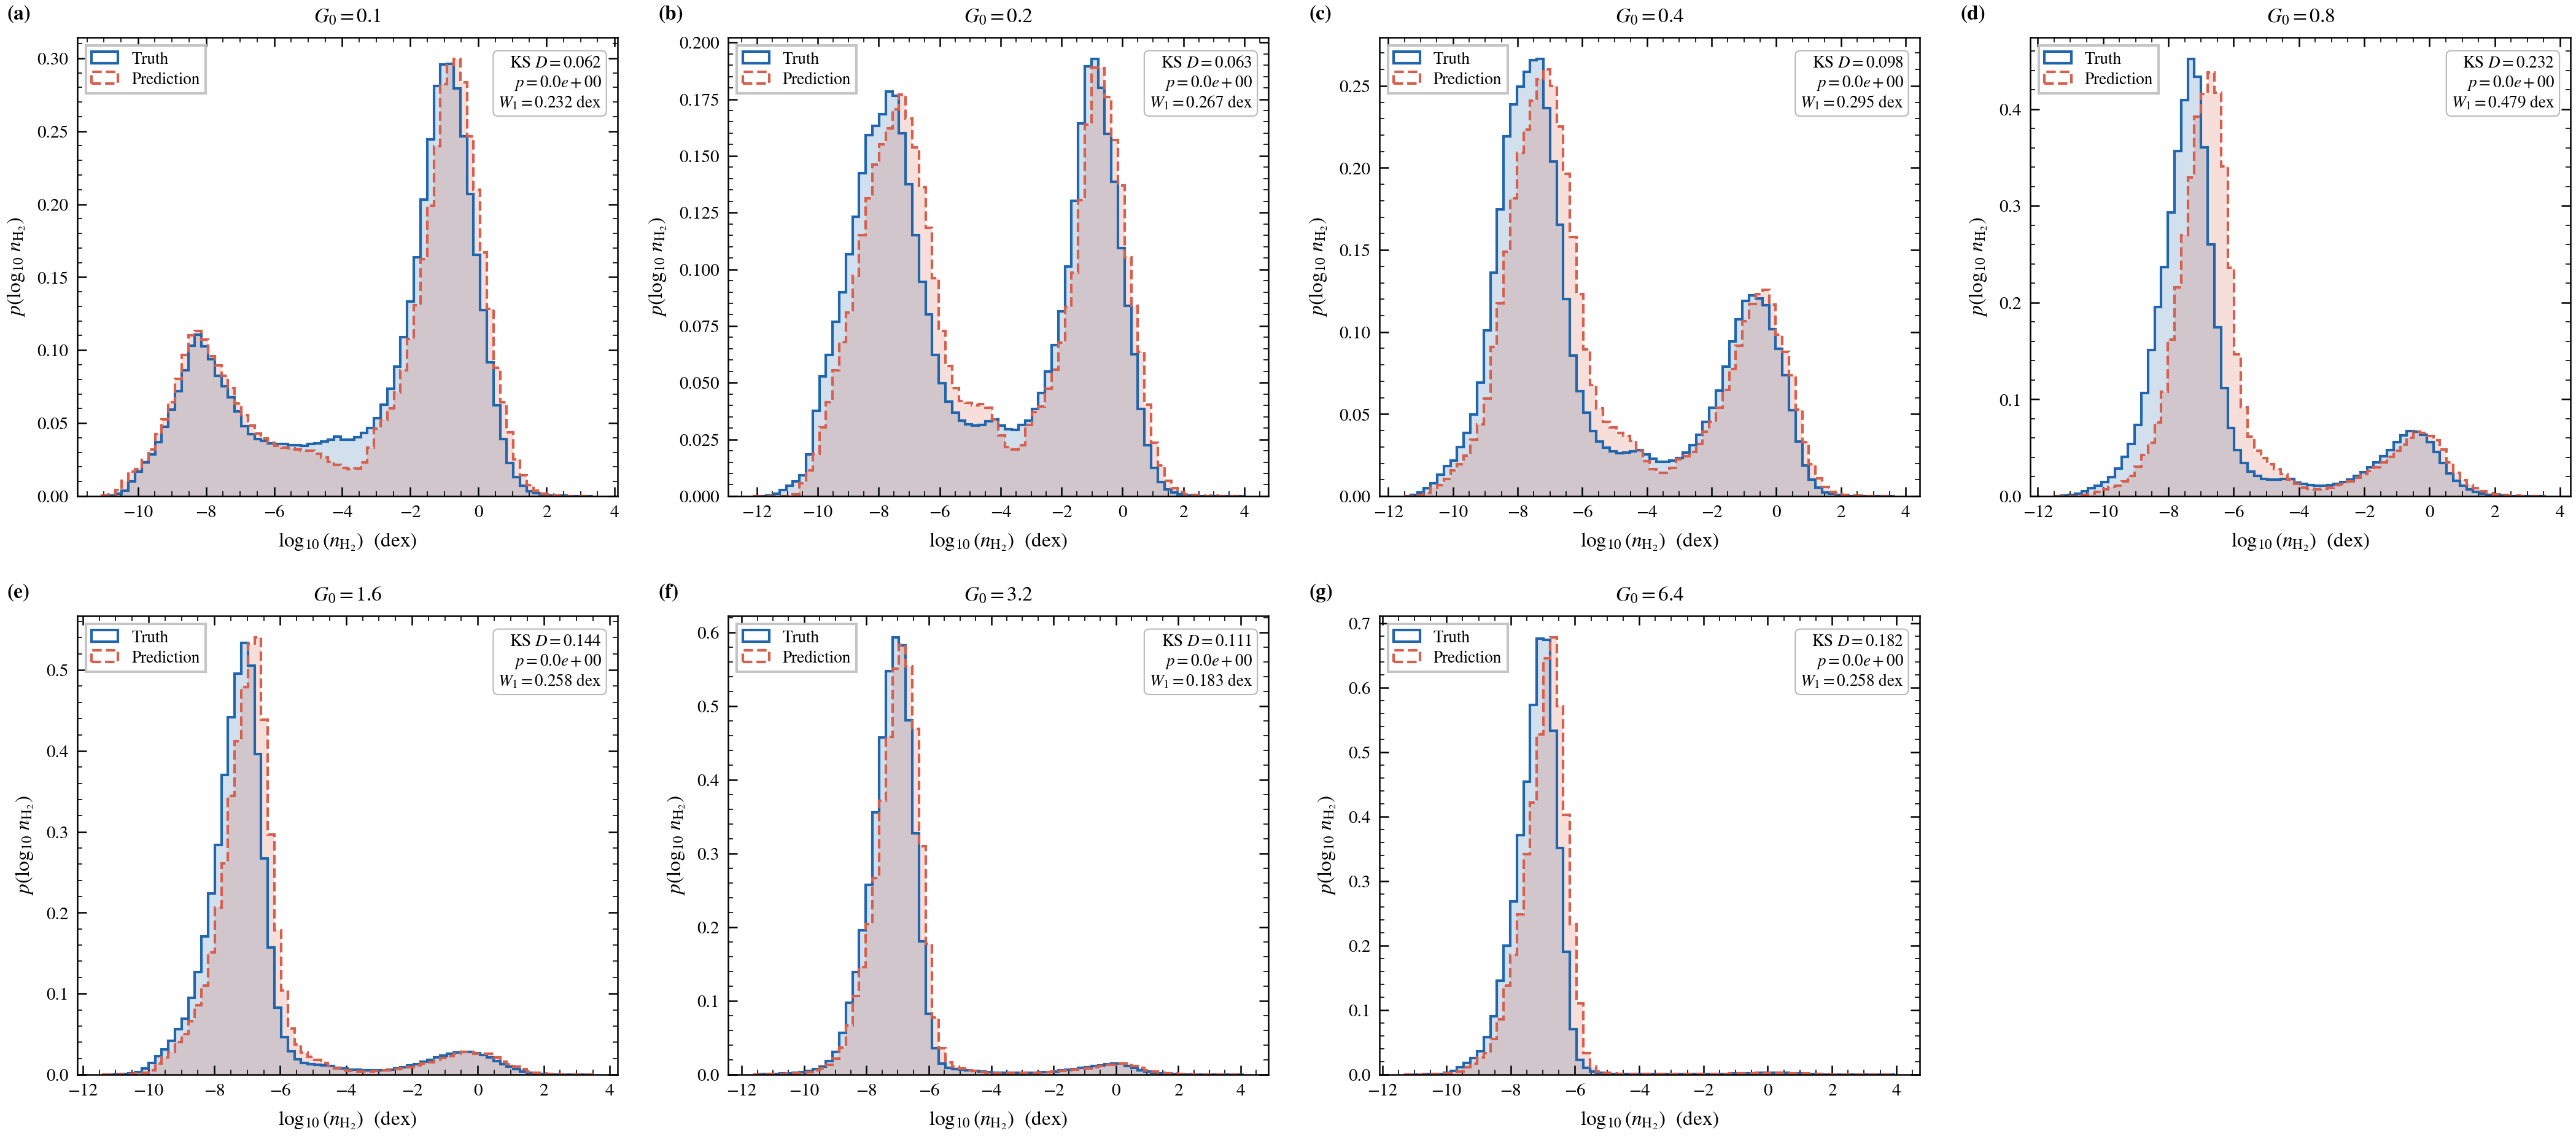
\includegraphics[width=\textwidth]{analysis_output/fig6_distributions.png}
\caption{Marginal distributions of $\logn$: true (blue, filled) and
predicted (red, dashed outline) for each held-out fold. The ensemble
accurately reproduces the bimodal structure at low $\Gzero$ and the
narrower UV-dominated distribution at high $\Gzero$. Per-fold $\Rsq$,
KL divergence, and MAE are annotated in each panel.}
\label{fig:distributions}
\end{figure*}

\subsection{Ensemble comparison}
\label{sec:results_ensemble}

The equal-weight ensemble \enssp{} (mean $\Rsq = 0.948$) marginally but
consistently outperforms the Ridge meta-learner \textsc{stacked\_sp}
(0.946). With only seven training folds, the meta-learner does not have
sufficient meta-training signal to learn combination weights that
transfer reliably to every held-out fold; equal averaging is the more
robust choice in this low-fold-count regime. Including the 3D U-Net in
any ensemble consistently \emph{lowers} the mean $\Rsq$: the
\textsc{ens\_xgb+cnn} configuration achieves 0.897, worse than
\textsc{xgb\_standard\_sp} alone (0.924), because in the folds where
the CNN predicts $\Rsq < 0$, averaging with a well-calibrated tabular
predictor degrades the result.

\subsection{Spatial structure of predictions}
\label{sec:spatial_preds}

Figure~\ref{fig:spatial} shows representative 2D slices of the
$\logn$ field. At low $\Gzero$ the field displays rich filamentary
spatial structure driven by self-shielding, with sharp transitions at
cloud boundaries; at high $\Gzero$ the field is nearly uniform and
residuals are minimal. This contrast explains the asymmetric difficulty
of the boundary folds: the low-$\Gzero$ self-shielding morphology
involves spatial gradients absent from the mid-range training cubes,
while the high-$\Gzero$ UV-dominated morphology is a smooth continuation
of the trend visible across the training range.

\begin{figure*}
\centering
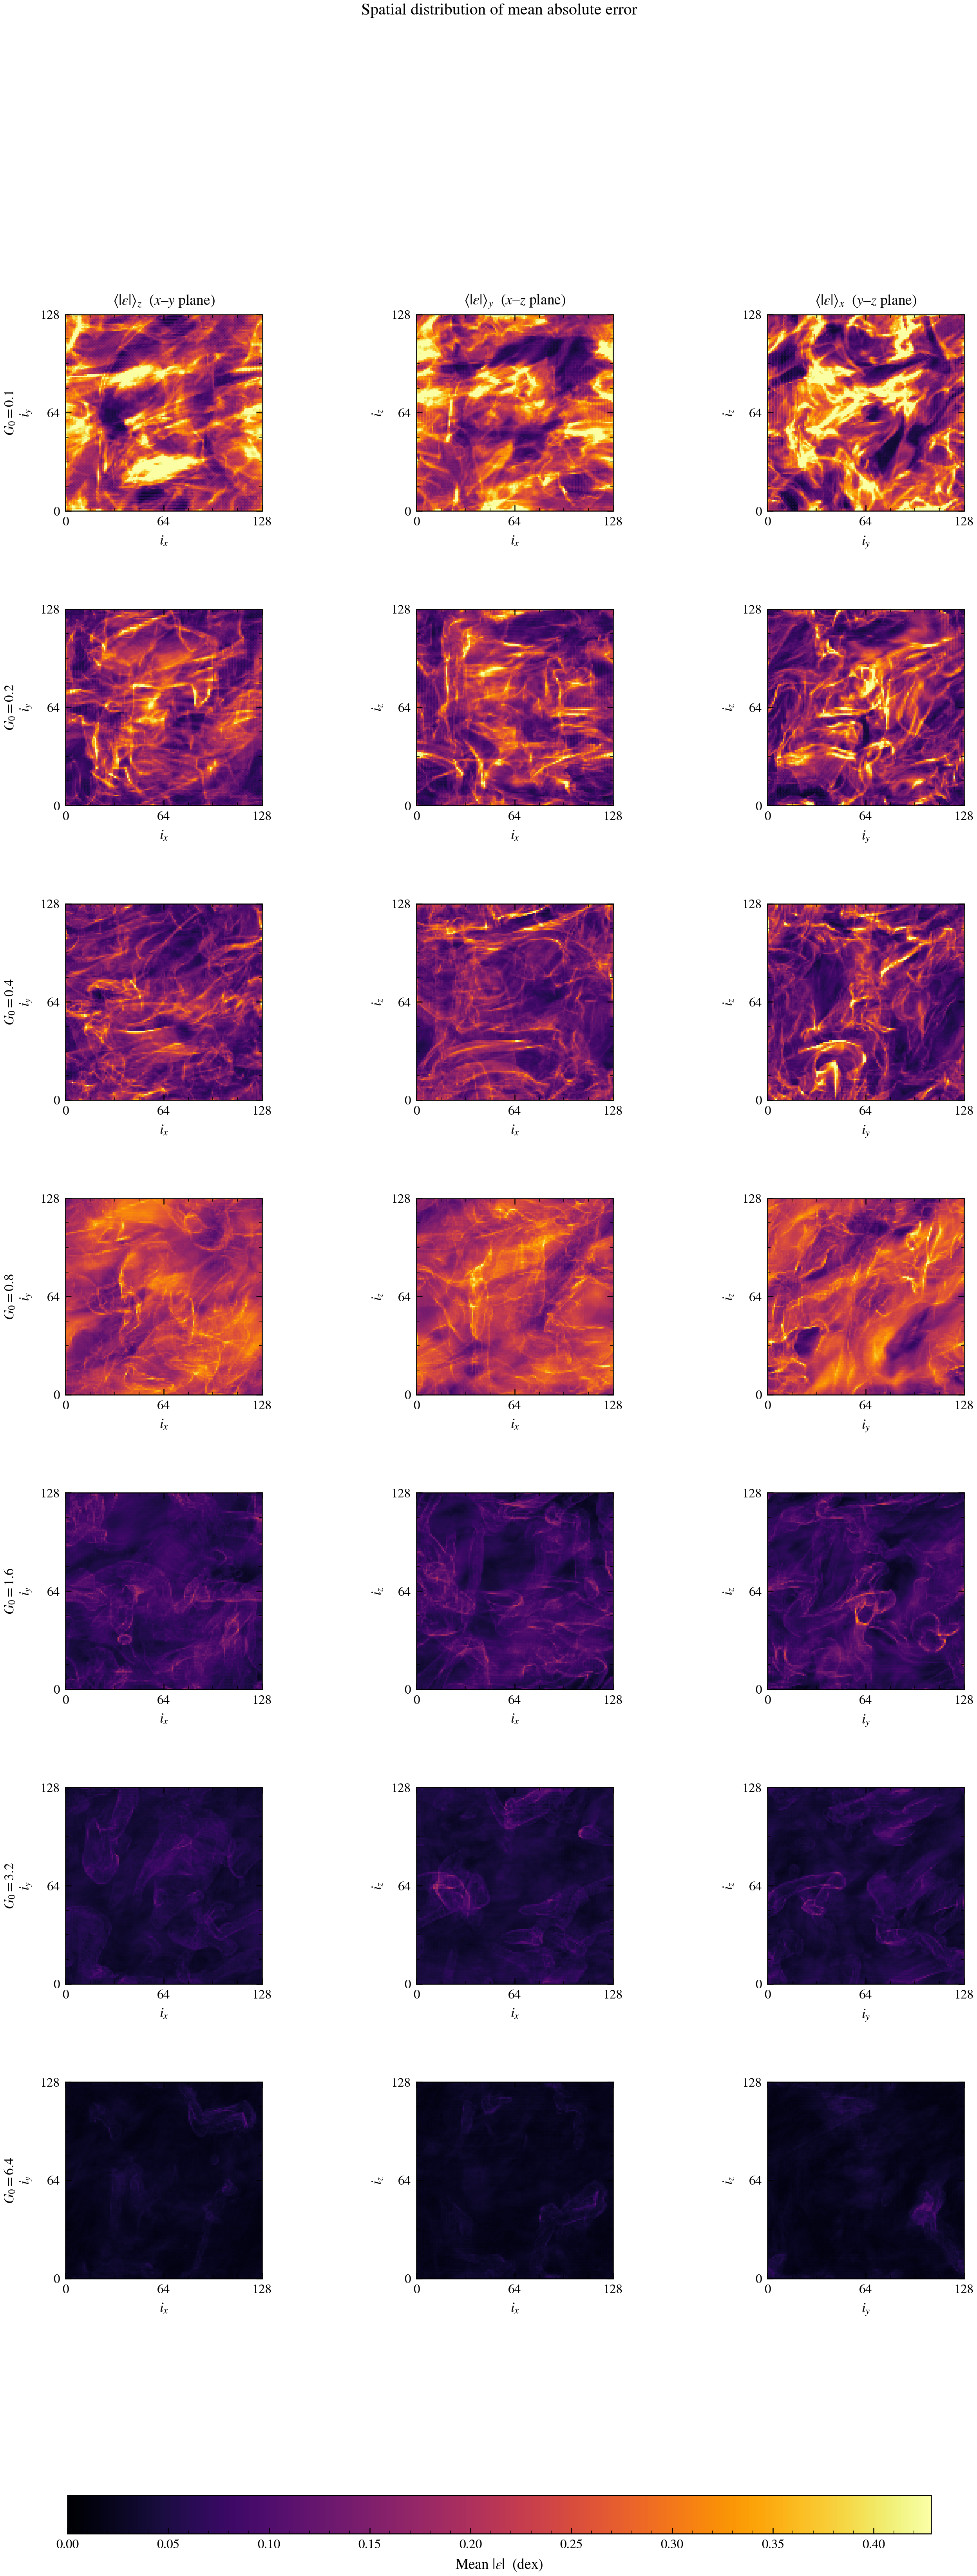
\includegraphics[width=\textwidth,height=0.85\textheight,keepaspectratio]{analysis_output/fig5_spatial.png}
\caption{Representative 2D mid-plane slices of the $\logn$ field across
all seven $\Gzero$ values. Each row shows the ground truth, prediction,
and absolute error (columns) for one fold. At low $\Gzero$ (top rows)
the field has rich filamentary structure and residuals are elevated at
cloud boundaries. At high $\Gzero$ (bottom rows) the field is nearly
uniform and residuals are small. Colour encodes $\logn$ on a common
scale.}
\label{fig:spatial}
\end{figure*}

% ============================================================
\section{Supplementary experiments}
\label{sec:supp}

\subsection{Single-cube extrapolation: knowledge transfer across \texorpdfstring{$\Gzero$}{G0}}
\label{sec:single_cube}

To quantify the information content of a single simulation and validate
the cross-validation design, we train \textsc{stacked\_sp} on each
individual cube and predict all seven, producing a $7 \times 7$ matrix
of log-space $\Rsq$ values in which rows index training cubes and columns
index test cubes.

Figure~\ref{fig:heatmap} shows these matrices for XGBoost, MLP, and the
stacked ensemble. The diagonal elements (in-sample fit) reach $\Rsq
\approx 0.99$. Off-diagonal elements decay monotonically with $\Gzero$
distance: one geometric step apart ($\times 2$ in $\Gzero$), $\Rsq
\approx 0.97$; two steps, $\approx 0.96$; three steps, $\approx 0.88$;
four steps, $\approx 0.75$; five steps, $\approx 0.45$; six steps
(i.e.\ $\Gzero = 0.1$ to $\Gzero = 6.4$), $\Rsq \approx 0.15$. The mean
off-diagonal $\Rsq$ across all 42 transfer pairs is approximately 0.78.

\begin{figure*}
\centering
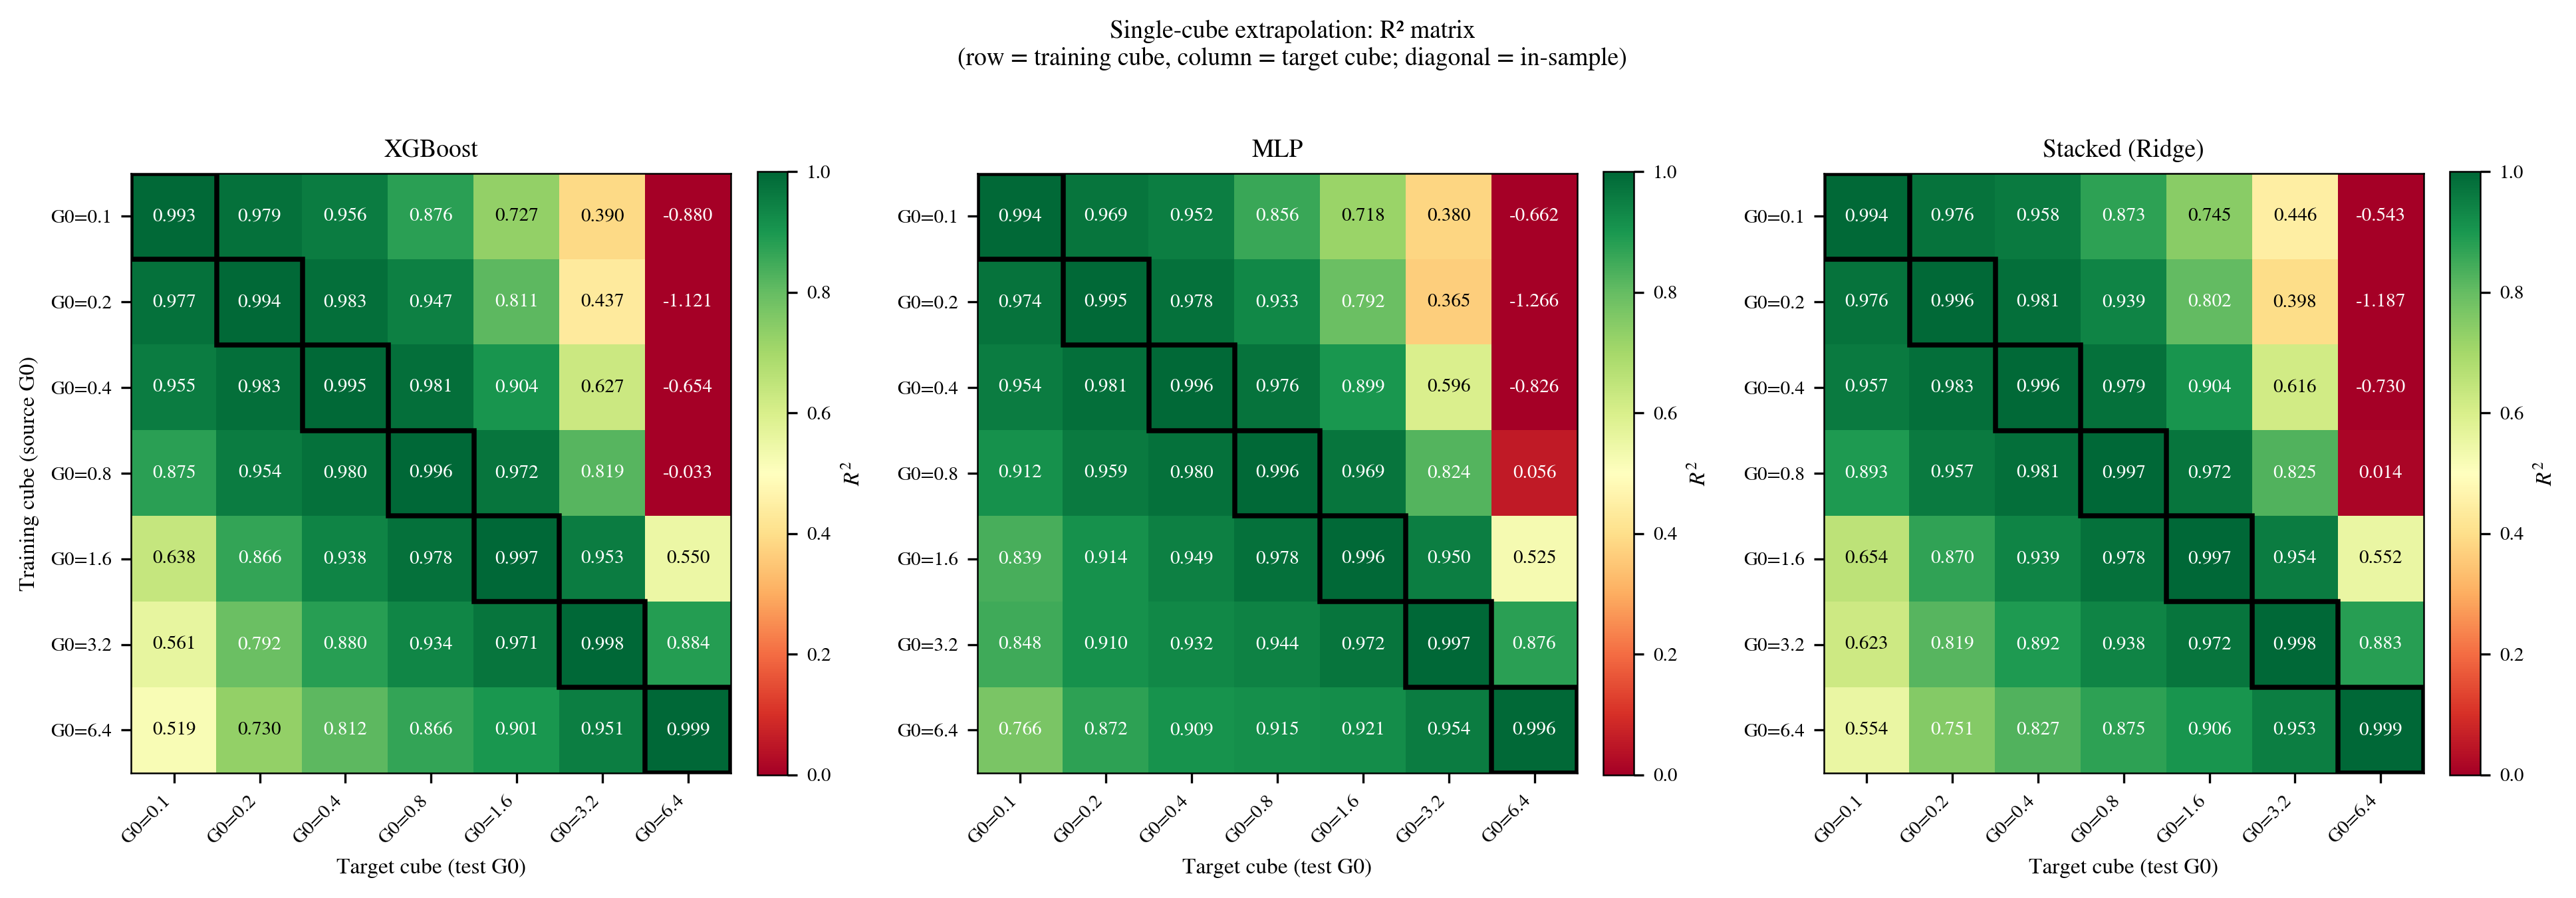
\includegraphics[width=\textwidth]{logs/single_cube_extrapolation/heatmap_20260313_022129.png}
\caption{Single-cube extrapolation: $7 \times 7$ log-space $\Rsq$
matrices for XGBoost (\emph{left}), MLP (\emph{centre}), and stacked
ensemble (\emph{right}). Rows index training cubes; columns index test
cubes; the diagonal (bold outline) gives in-sample fit ($\Rsq \approx
0.99$). Colours range from red ($\Rsq < 0$) through white (0.5) to
green ($\Rsq > 0.9$). Off-diagonal values decay monotonically with
$\Gzero$ distance: chemical knowledge transfers well within $\times 4$
in $\Gzero$ but degrades rapidly at larger separations.}
\label{fig:heatmap}
\end{figure*}

The local chemical equilibrium --- the mapping from density, temperature,
and shielding proxies to $\nHH$ --- is approximately universal within a
$\Gzero$ ratio of 4--8 but breaks down over larger factors. This is
consistent with the physical picture that the H$_2$ formation and
photodissociation rate functions are universal; what changes across
$\Gzero$ is the equilibrium balance point. The result validates the
leave-one-$\Gzero$-out design by showing that a single-cube model is
qualitatively weaker than the six-cube training ensemble, and that none
of the 64-fold UV range is redundant in the training set.

\subsection{Intra-cube spatial section: observational survey design}
\label{sec:intra_cube}

We ask whether the \enssp{} surrogate can reconstruct the $\nHH$ field
within a single simulation from partial spatial coverage, and whether the
\emph{geometry} of the observed fraction matters more than its volume.
For each of the seven $\Gzero$ cubes, we train \textsc{stacked\_sp} on a
spatial subset of cells and evaluate on the complement, testing three
sampling geometries at varying coverage fractions.

In the \emph{random} configuration, cells are sampled uniformly at
random, preserving the statistical distribution of local physical
conditions across the training set. In the \emph{contiguous slab}
configuration, all cells from one spatial half of the cube along a
coordinate axis are used for training. In the \emph{contiguous box}
configuration, a compact cubic sub-region of specified volume fraction is
used.

Figure~\ref{fig:intra_cube} shows the test $\Rsq$ as a function of
geometry and coverage fraction for all seven $\Gzero$ cubes. The results
are striking. A randomly sampled 1 per cent of cells ($\approx$21\,000
cells) achieves test $\Rsq = 0.897$ on the remaining 99 per cent.
Increasing the fraction to 5, 10, 25, and 50 per cent yields $\Rsq$ of
0.952, 0.963, 0.970, and 0.980 respectively. By contrast, a contiguous
slab covering 50 per cent of the volume --- 23 times as many cells as
the 1 per cent random sample --- yields test $\Rsq = -0.394$ (x-axis
slab), $-2.689$ (y-axis), and $-1.389$ (z-axis).

\begin{figure*}
\centering
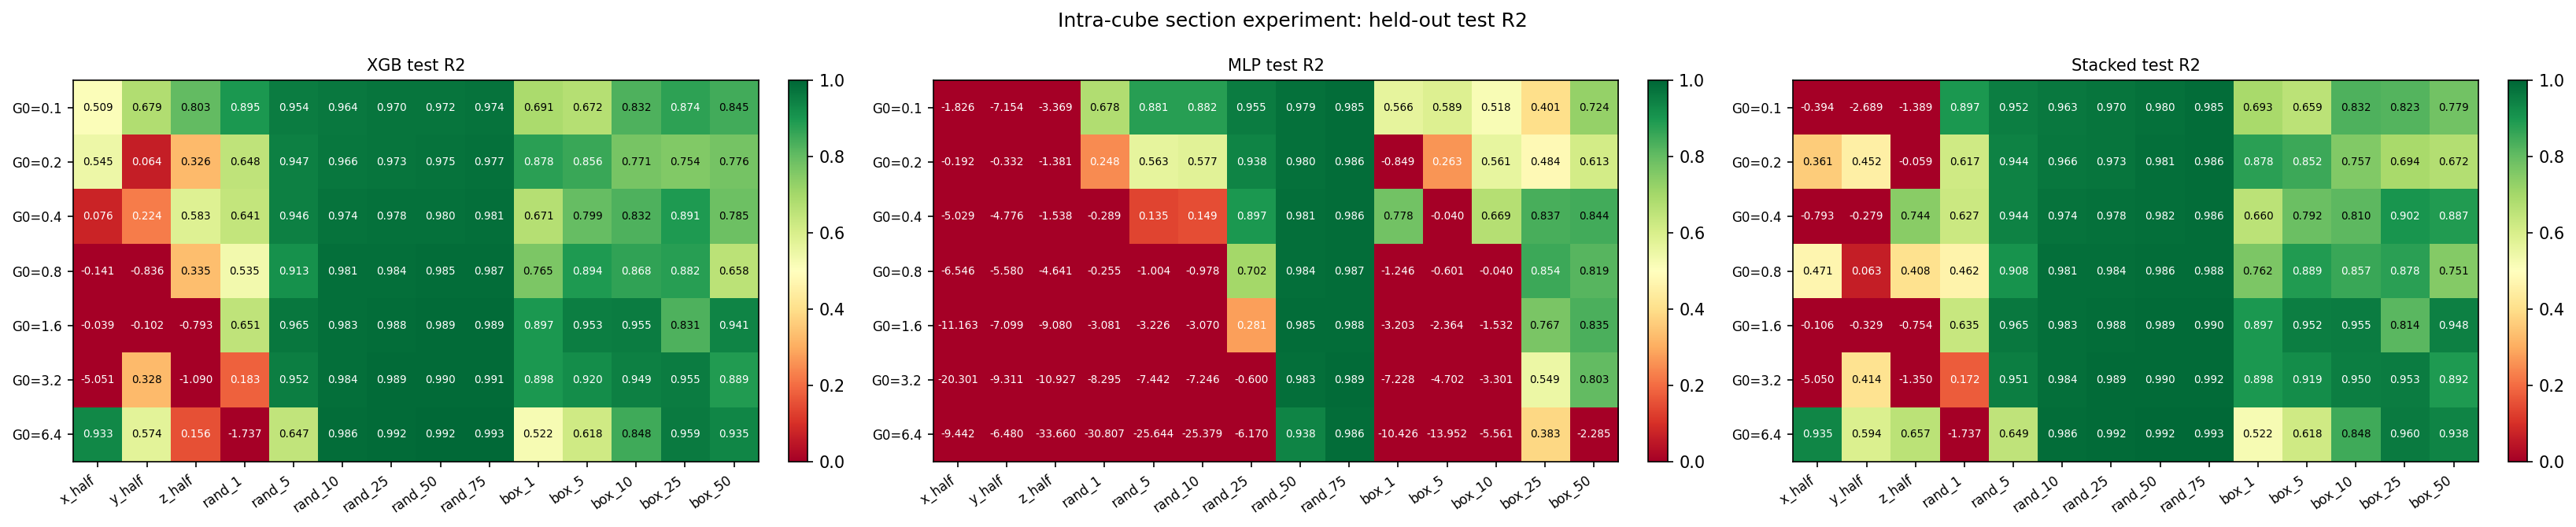
\includegraphics[width=\textwidth]{logs/intra_cube_section/run_20260313_142443_heatmap.png}
\caption{Intra-cube spatial section: test $\Rsq$ as a function of
training geometry (columns) and source $\Gzero$ (rows) for XGBoost
(\emph{left}), MLP (\emph{centre}), and stacked ensemble (\emph{right}).
Random sampling at 1 per cent achieves $\Rsq \approx 0.90$ (green);
contiguous slabs at 50 per cent coverage achieve $\Rsq \ll 0$ (red),
worse than predicting the training mean at every test cell. Contiguous
boxes are intermediate. The pattern is consistent across all seven
$\Gzero$ values.}
\label{fig:intra_cube}
\end{figure*}

The mechanism is the behaviour of the spatial neighbourhood features
under different geometries. With random sampling, every test cell has
training cells nearby in all three spatial dimensions; the box-filter
neighbourhood features, computed from training cells, provide meaningful
local averages for each test cell even at 1 per cent coverage. With
contiguous-slab training, the model is trained exclusively on the
UV-illuminated surface of the cloud and cannot correctly predict the
shielded interior: the feature distributions of interior cells fall
entirely outside the training distribution, and the model defaults to an
extrapolated mean that is systematically wrong. The z-axis slab is less
catastrophic than the transverse slabs (z $\Rsq = -1.4$ versus $-2.7$
for y) because the UV illumination direction along z produces a smoother
gradient from surface to interior, making the half-cube feature
distribution slightly more representative.

The practical consequence for observational astronomy is that an H$_2$
density field can be reconstructed from a sparse set of uniformly
distributed sight-line observations --- the kind obtainable from an
integral field unit (IFU) spectrograph with a sparse sampling grid ---
with $\Rsq \approx 0.90$ at only 1 per cent spatial coverage. Deep,
contiguous mapping of a single region consumes far more observing time
while providing negligible reconstruction accuracy. Efficient H$_2$
density surveys should prioritise coverage uniformity over observational
depth.

% ============================================================
\section{Discussion}
\label{sec:discussion}

\subsection{Feature engineering versus architecture search}

The central methodological lesson of this work is that feature
engineering dominates model architecture as a source of performance gain.
The +0.031 $\Rsq$ improvement from the $3^3$ spatial features is larger
than any architecture change, and the full multi-scale extension to
three kernel sizes (+0.038 combined) exceeds the ensemble gain (+0.024).
This is consistent with the finding of \citet{Grinsztajn2022} that
tree-based models with engineered features routinely outperform deep
learning on tabular regression problems when training data volume is
limited. The specific features chosen here --- uniform box-filter means
--- are the simplest possible representation of spatial context; more
sophisticated descriptors (local gradients, anisotropic kernels aligned
with the UV illumination axis) could in principle improve accuracy
further, particularly for the extrapolation folds.

\subsection{Volumetric versus per-cell representations}

The 3D U-Net has the nominally correct inductive bias for a spatially
correlated field: its hierarchical receptive field should, in principle,
learn to aggregate the shielding column density in a physically
meaningful way. In practice, the mismatch between volumetric sample count
(48 augmented cubes) and model parameters (5.8\,M for
\textsc{unet\_standard}) prevents the development of generalizable
spatial representations, and the additional resolution loss from
downsampling ($128^3 \to 64^3$) discards the fine-scale gradients at
cloud boundaries where $\nHH$ varies most sharply. This identifies a
general principle for simulation emulation with limited data: the choice
between volumetric and per-cell approaches should be governed by the
training sample-to-parameter ratio, not the nominal spatial nature of
the problem. Volumetric models become competitive when dozens to hundreds
of high-fidelity simulation volumes are available.

\subsection{Regularisation in the limited-parameter regime}

The catastrophic failure of dropout in the extrapolation folds reflects a
tension between standard regularisation wisdom and the requirements of
physical extrapolation. Dropout prevents overfitting by forcing redundant
feature representations, which is beneficial when the model is
memorising noise. In this problem, where the model must form coherent
representations of a physical process over only six discrete $\Gzero$
training values, dropout prevents the \emph{structure} of the learned
representation from being preserved under extrapolation. This finding may
be relevant to other simulation emulation contexts where training covers
only a small number of discrete parameter values.

\subsection{Limitations}

Several limitations apply. The UV-only suite models chemistry under a
spatially uniform, time-steady UV field; real molecular clouds experience
anisotropic and time-varying radiation from nearby massive stars. The
$z$-preserving augmentation strategy would require modification for
simulations with different illumination geometries. The feature set
includes $\log\fshield$, a non-local quantity computed from the full 3D
H$_2$ column density; in a deployment scenario where $\nHH$ is unknown,
$\fshield$ would need to be estimated from other tracers, and that
uncertainty would propagate into the $\nHH$ prediction. Finally, the
data set represents a single turbulent ISM realisation at each $\Gzero$
value; generalisation across different initial conditions, magnetic field
strengths, and density regimes remains to be quantified.

% ============================================================
\section{Conclusions}
\label{sec:conc}

We have developed and systematically evaluated ML surrogates for the
molecular hydrogen number density in 3D ISM simulations, using
leave-one-$\Gzero$-out cross-validation to measure out-of-distribution
generalisation across the dominant physical parameter. Our main
conclusions are as follows.

(i) An equal-weight ensemble of XGBoost and a wide MLP, each trained on
a 60-dimensional feature vector combining 15 local physical fields with
45 multi-scale spatial neighbourhood averages (kernel sizes $3^3$, $5^3$,
$7^3$), achieves a mean log-space $\Rsq$ of $0.948 \pm 0.024$ across
seven leave-one-$\Gzero$-out folds, with a minimum per-fold $\Rsq$ of
0.908 at the hardest extrapolation fold ($\Gzero = 0.1$).

(ii) The single largest performance improvement (+0.031) comes from
adding $3^3$ spatial neighbourhood features, not from any model
architecture change. Neural architecture search (three MLP designs, three
XGBoost depths) yields differences smaller than 0.003.

(iii) A 3D U-Net CNN achieves a best mean $\Rsq$ of $0.803 \pm 0.172$
with an order of magnitude greater fold-to-fold variance, owing to the
mismatch between volumetric training sample count (48 augmented cubes)
and model parameters (5.8\,M). Including the CNN in any ensemble reduces
the mean $\Rsq$.

(iv) Dropout regularisation catastrophically degrades extrapolation to
unseen $\Gzero$ values when training covers only six discrete UV field
strengths. L2 weight decay is the appropriate regulariser in this regime.

(v) Per-fold target normalisation (standardisation of $\logn$ per
training fold) is essential for CNN stability: without it, $\Rsq < 0$;
with it, $\Rsq = 0.775$ immediately.

(vi) Single-cube extrapolation experiments confirm that chemical
knowledge transfers well over $\Gzero$ ratios up to $\sim\!4$--$8\times$
($\Rsq > 0.88$) but degrades rapidly over larger factors, validating the
leave-one-$\Gzero$-out protocol.

(vii) Intra-cube spatial sampling experiments demonstrate that 1 per cent
uniform random coverage reconstructs the $\nHH$ field with $\Rsq =
0.897$, while 50 per cent contiguous-slab coverage yields $\Rsq = -0.394$.
Coverage uniformity is the critical design parameter for observational
H$_2$ density surveys; surveys targeting molecular cloud sight-lines
should prioritise spatial uniformity over contiguous depth.

The \enssp{} surrogate predicts $\nHH$ at all 2,097,152 cells of a
$128^3$ cube in seconds on a single GPU, with accuracy within
\(\sim\!0.1\)--\(0.2\)\,dex of the self-consistent simulation value across a
64-fold UV field range.

% ============================================================
\section*{Acknowledgements}

The author thanks the developers of XGBoost, PyTorch, NumPy, SciPy, and
Matplotlib for the open-source tools on which this work depends.

\section*{Data availability}

All trained model outputs, prediction arrays, and experimental logs are
archived as timestamped JSON and \texttt{.npz} files. The full pipeline
is deterministic and runs end-to-end on a single consumer GPU.

% ============================================================
\bibliographystyle{mnras}
\bibliography{references}

\label{lastpage}
\end{document}
